\documentclass{article}

\usepackage{packages}
\usepackage{environments}
\usepackage{commands}

\begin{document}

\title{Typing Analysis}
\author{Dima Trushin}
\date{}
	
\maketitle
\tableofcontents

\newpage

\section{General information}

The application uses Qt environment as an ecosystem. It does not use RTTI (however, Qwt library uses RTTI) and uses exceptions. Application uses static linking and presents a single binary file as a result. All components of the program must be inside \verb"NSApplication" namespace. Nested namespaces should be placed in a subfolder of the project.

\subsection{Addressable objects}

I use a notion of an addressable object. It means an object that has a constant address during its life-time and can be referenced by other objects. There are several types of addressable objects:
\begin{enumerate}
\item \verb"QObject".
\item \verb"CApplicationImpl" or any other implementations located on the heap (PIMPL).
\item Observer/Observable.
\end{enumerate}
Addressable objects must be created on the heap via \verb"std::make_unique" or similar mechanism. An exception to this rule: you may create an addressable object inside another addressable object.

\subsection{Exceptions}

The strategy is to catch an exception, show a message, and die. Since Qt environment is not totally exception safe, it is not allowed to throw exceptions in an event loop. If a \verb"QObject" requires to throw an exception and terminate the program it catches the exception by itself and then sends a signal to \verb"CQtLoopException" object. \verb"CQtLoopException" shows the exception message and stops the event loop. \verb"CQtLoopException" is a singleton, it uses \verb"CAnyGlobalAccess" template (see~\ref{section::Singleton}).

\section{Application behavior}

The global logic of the entry point is the following:
\begin{enumerate}
\item Application acquires all the required resources.
\item Application starts the Qt event loop.
\end{enumerate}

When started the application intercepts keyboard events system-wide, translates them into OS independent form and sends them into the kernel of the application. If debugging macros are enabled (see~\ref{section::Debugging}), additional debugging windows are shown to output debug information.

\verb"KeyboardHandler" is an object intercepting the keyboard system-wide. It notifies the kernel of the application about key pressing and releasing. The kernel computes the required information and notifies the interface of the application. From the other hand the interface elements control the kernel. All elements of the kernel are connected using Observer pattern~\ref{section::Observer}. The interface and the kernel are connected using MVC pattern. The MVC pattern is based on the Observer pattern as written \href{https://stlab.cc/tips/about-mvc.html}{here} by Sean Parent.

\section{Application Structure}

\subsection{Overview}

\verb"CApplication" object initializes all required resources for the application including the ones to interact with Qt ecosystem. It may throw an exception while constructing. In order to minimize stack usage \verb"CApplication" contains \verb"std::unique_ptr" to \verb"CApplicationImpl" (it is an addressable object). \verb"CApplicationImpl" consists of four parts:
\begin{enumerate}
\item \verb"CApplicationGlobals". Its purpose is to initialize global resources, e.g., timers, loggers, thread pools, etc. Application initializes all global resources (basically singletons) at the start. This allows not to wast time on the first call. Also, it is inconvenient to initialize timers via the first call.

\item \verb"CApplicationKernel". Its purpose is to initialize the kernel of the application. The kernel does not depend on the GUI and uses MVC via observer pattern to interact with GUI.
\item \verb"CApplicationGUI". Its purpose is to provide View wrappers over Qt resources compatible with MVC pattern.

\item \verb"CApplicationImpl". Its purpose is to connect the kernel and the GUI via MVC.
\end{enumerate}
The order of construction is ensured by the inheritance mechanism.
\begin{center}
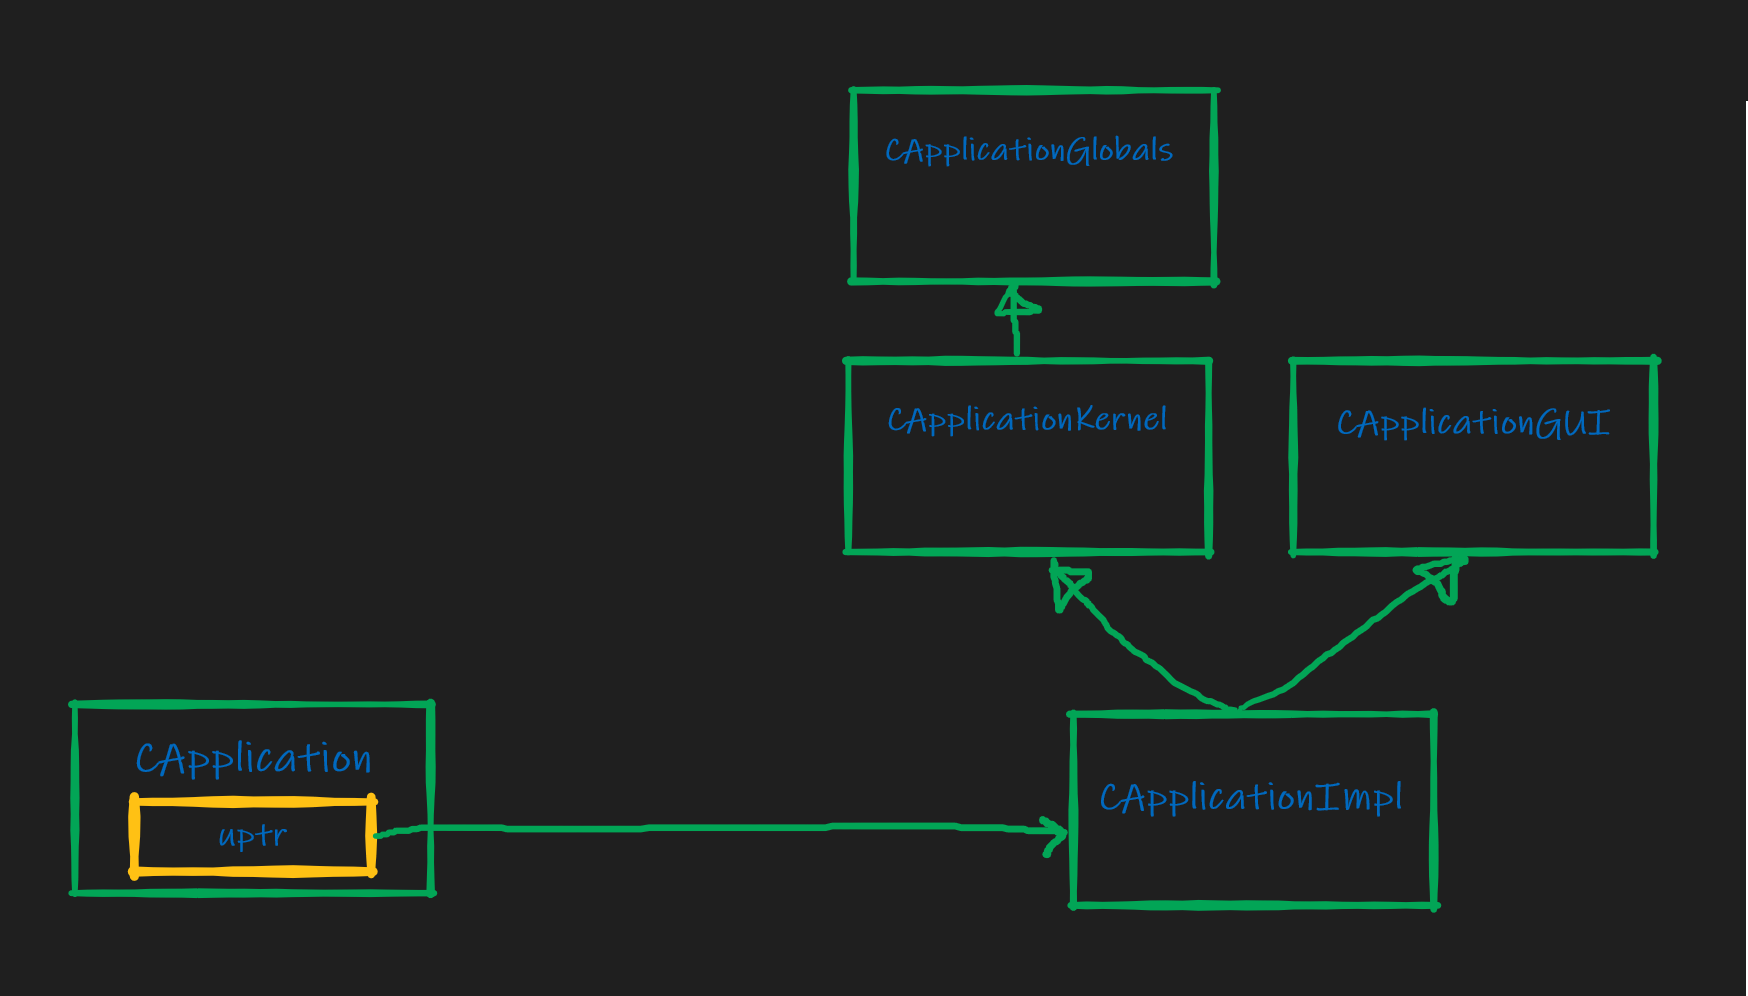
\includegraphics[scale = 0.3]{Figures/CApplicationStructure.png}
\end{center}

\subsection{Application data flow}

Currently the following modules are implemented.

\begin{center}
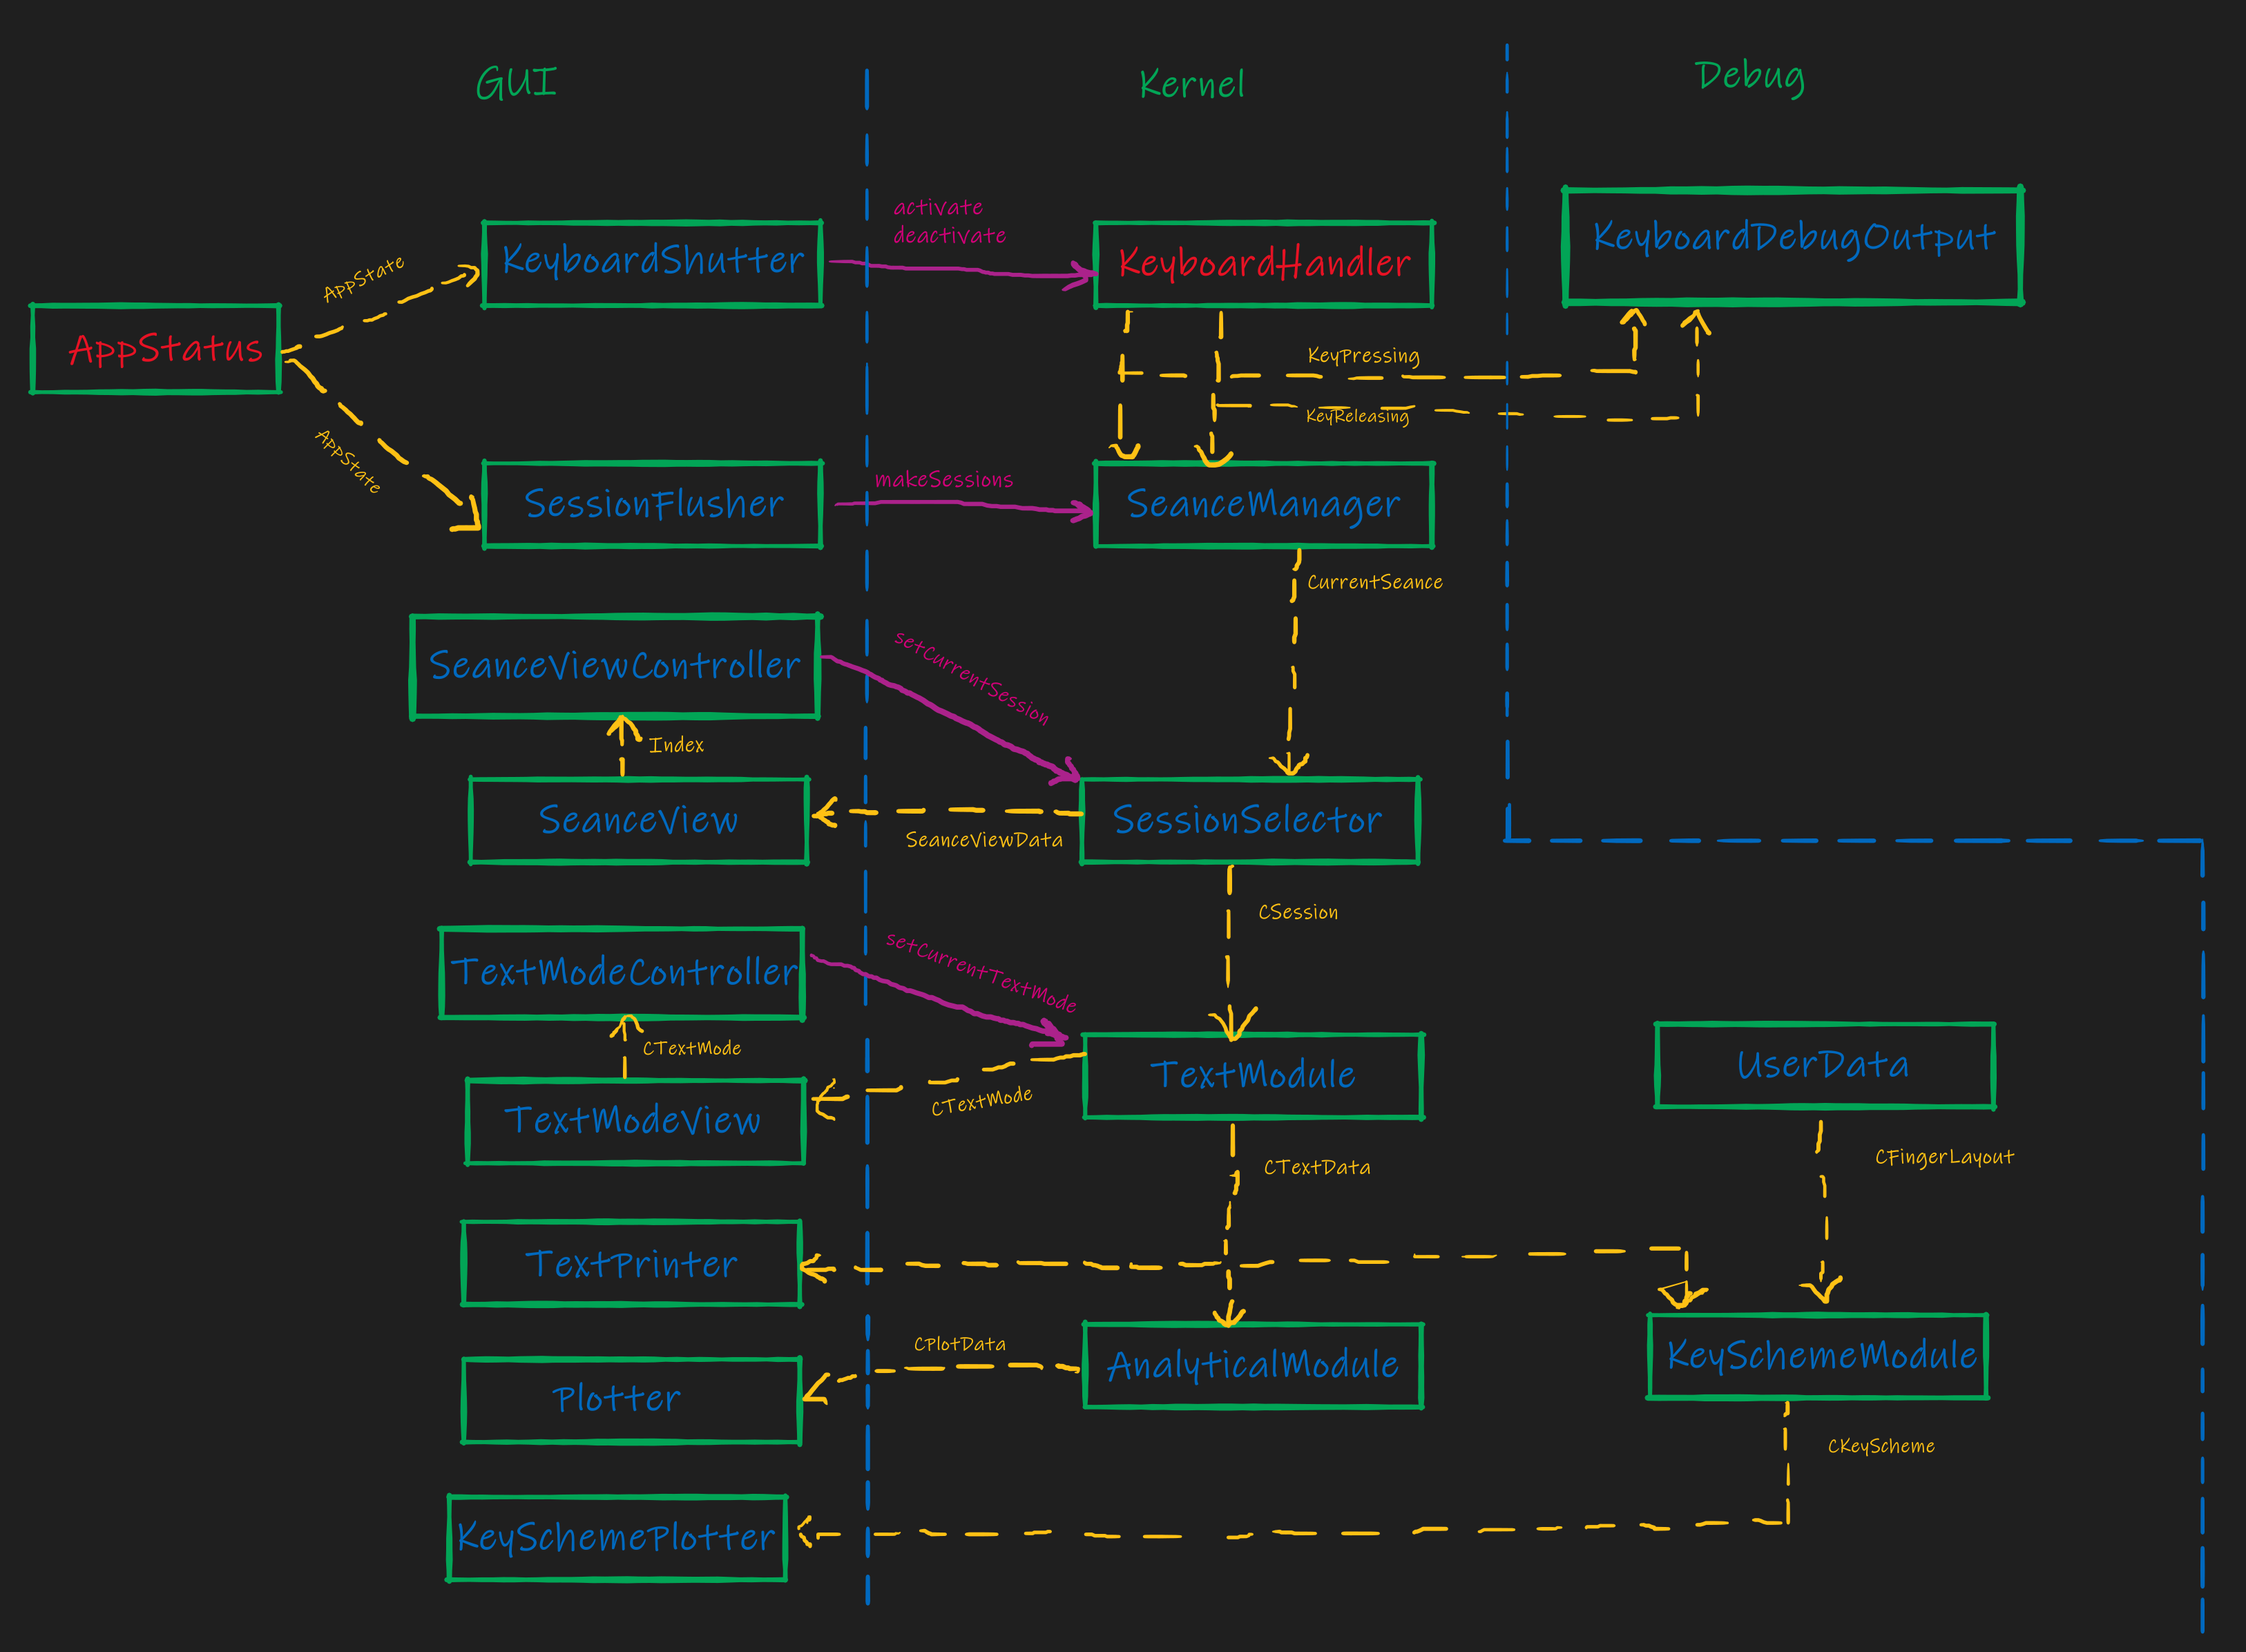
\includegraphics[scale = 0.4]{Figures/Modules.png}
\end{center}

The boxes are application components. Red color means that the objects are global and blue color means that the objects are local. Yellow lines denote Observable/Observer relationship. Violet lines represent Control/Model relationship. The arrows denote the direction of the data flow.


\subsection{Keyboard}

Each key on a keyboard has its position identifier \verb"CKeyPosition" and a key identifier \verb"CKeyId". \verb"CKeyPosition" points out a physical location on a keyboard (e.g. a row and a column where the key is located). \verb"CKeyId" identifies the key depending on the keyboard layout (qwerty, Dvorak, etc.) \verb"CKeyPosition" is an enum with the following identifiers (xkb identifiers):
\begin{center}
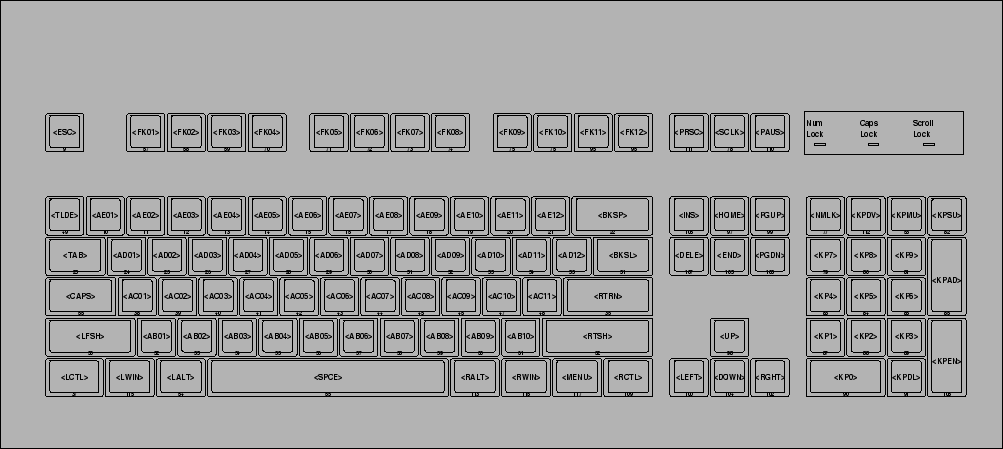
\includegraphics[scale = 1]{Figures/KeyPosition.png}

The picture is taken from \href{https://www.charvolant.org/doug/xkb/html/node5.html}{here}
\end{center}
It should be noted that the numeric values of the identifiers are slightly different from the ones in xkb.

\subsection{Keyboard Interception}

The application must intercept keyboard events system-wide even if application is on the background. Qt ecosystem does not allow doing this. Hence, we need to implement our own mechanism. System wide interception usually means that raw keyboard data is being intercepted. Hence, we need to implement translation of the key events to generated text. The main problem here is dead keys and ligatures (left directional and bidirectional text is not supported in any way, shape, or form). Current implementation supports dead keys but not ligatures (but the design allows to extend implementation to ligatures TO DO). Since system-wide interception must be done on the level of current OS, we implement this mechanism separately for each supported OS. Currently the list of the supported OS is the following
\begin{enumerate}
\item Windows 8 or higher.
\item Linux with X11 (there is a working prototype, not implemented yet, need to specify all the details TO DO).
\item macOS 10.14 (Mojave) or higher (there is a working prototype, not implemented yet, need to specify all the details TO DO).
\end{enumerate}

\paragraph{Current design}

The design is based on ideas of \href{https://github.com/asokol123}{Alexey Sokolovsky}. He is also in charge of Linux and macOS implementations.

The main object here is \verb"CKeyboardHandler". It serves as an object receiving all key events in a system independent form. This is a singleton described in section~\ref{section::KeyboardHandler}. Let us consider the following figure:
\begin{center}
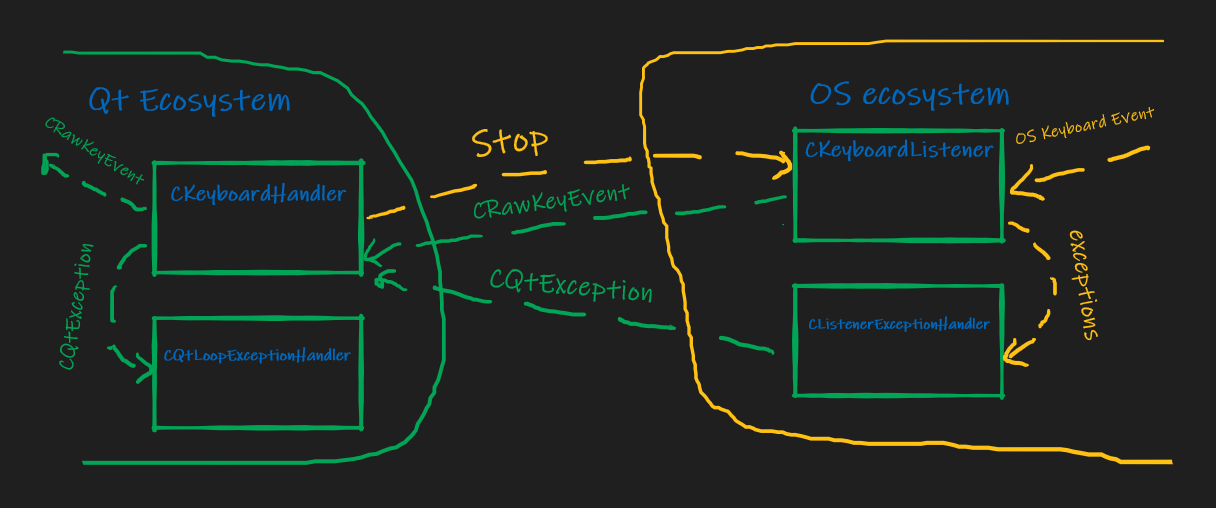
\includegraphics[scale = 0.5]{Figures/KeyboardInterception.png}

Green arrows represent queued Qt signals and yellow arrows represent OS dependent signals.
\end{center}

\verb"CKeyboardHandler" acts on the main GUI thread. It lives in Qt ecosystem and spawns an additional thread while construction. This additional thread lives in the OS ecosystem. 

\paragraph{CKeyboardListener}
The main object acting on the additional thread is \verb"CKeyboardListener". Its roles are:
\begin{enumerate}
\item Intercept key events system-wide.

\item Extract all the information from OS key events and translate them to OS independent form.

\item Resend OS independent key events to \verb"CKeyboardHandler" via Qt event system.

\item It receives only one message from \verb"CKeyboardHandler" via OS ecosystem message system. This is a ``stop'' message. Receiving the message, it stops the additional thread.
\end{enumerate}

There are two types of messages sent by \verb"CKeyboardListener":
\begin{enumerate}
\item Key pressing message.
\item Key releasing message.
\end{enumerate}
Key pressing message contains more information.

\paragraph{CListenerExceptionHandler}
The second object acting on the additional thread is \verb"CListenerExceptionHandler". Its roles are:
\begin{enumerate}
\item Extract exception information.
\item Resend special exception messages to \verb"CKeyboardHandler".
\end{enumerate}
If an exception happens the event loop on the additional thread stops. \verb"CKeyboardHandler" resend the message to \verb"CQtEventLoopExceptionHandler". The latter one shows the error message and terminates the program.


When we need to shut down the keyboard interception temporary, we make \verb"CKeyboardHandler" to ignore the messages from \verb"CKeyboardListener". The latter object is always on and operational.

\subsection{System independent Key event}

The \verb"CKeyEvent" contains the following information:
\begin{enumerate}
\item Pressing time.

\item Releasing time.

\item \verb"CKeyPosition" is an identifier of the Key position on the keyboard (independent on the layout, this is a physical instance of a key). It identifies the key uniquely.

\item \verb"CKeyId" is an identifier of the Key depending on the layout being used. It is based on the Windows Virtual Key table.

\item \verb"CLabelData". Key Label. This one describes how to label a key on the keyboard. It contains at most two \verb"QChar"s (the symbol for the key and the symbol for the key with shift being pressed).  For example, if a key is a letter or a number key, then the label contains two symbols. For system keys like shifts, backspace, enter, etc, the label information usually contains one special symbol.

\item \verb"CKeyTextData". Key Text. This is a sequence of symbols appearing after pressing this key. It can be $0$, $1$, or $2$ symbols. The exact rules are explained below.

\item Flags. The flags contain the following information:
\begin{enumerate}
\item The control keys (shift, ctrl, alt, capslock) that are active while the current key is pressed. If shift, ctrl, or alt flag is active, the control (shift, ctrl, or alt respectively) key was pressed. If capslock flag is active, the capslock key was toggled.

\item AutoRepeat flag marks the key if pressing was generated before releasing appeared. This means a synthetically generated pressing and not the actual key stroke.

\item DeadKey flag is active if the current key is a dead key.
\end{enumerate}
\end{enumerate}

\verb"CKeyboardHandler" receives the following structures from \verb"CKeyboardListener":
\begin{enumerate}
\item \verb"CKeyPressing".
\item \verb"CKeyReleasing".
\end{enumerate}

The structure \verb"CKeyPressing" contains the following fields:
\begin{enumerate}
\item \verb"CTime" The pressing time of the key.
\item \verb"CKeyPosition" The OS independent position of the key.
\item \verb"CKeyID" The OS independent ID of the key.
\item \verb"CLabelData". The key label information. These symbols are shown on the keyboard. It contains \verb"LowSymbol", \verb"HighSymbol", and \verb"Size" fields.
\item \verb"CKeyTextData". The text generated by the key. It contains \verb"Symbol[2]" array of \verb"QChar"s and \verb"Size" fields.
\item \verb"CKeyFlags". These flags show the control (shift, ctrl, alt, capslock) keys that are active while the current key is pressed.  If shift, ctrl, or alt flag is active, the control (shift, ctrl, or alt respectively) key was pressed. If capslock flag is active, the capslock key was toggled. Also it contains a dead key flag. The flag is active if the key is a dead key.
\end{enumerate}

The structure \verb"CKeyReleasing" contains the following fields:
\begin{enumerate}
\item \verb"CTime" The releasing time of the key.
\item \verb"CKeyPosition" The OS independent position of the key.
\item \verb"CKeyID" The OS independent ID of the key. (subject to change, probably need to exclude it TO DO)
\end{enumerate}

When we need to pair the pressing and releasing events into one key, we identify the key by its position. It should be noted that the ID of the key can change. For example, if we press a number on the numpad (and keep pressing), then press NumLock, and only then release the numpad number key, the numpad key will have different IDs while pressing and releasing. This happens because NumLock changes the mapping for physical keys to the corresponding IDs.

\subsection{Key mapping}

This section is mostly influenced by a \href{http://archives.miloush.net/michkap/archive/2006/03/23/558658.html}{series} of blogs by Michael S. Kaplan. His posts explain all subtleties of the keyboard handling on Windows. However, the principals he explains are applicable to any keyboard handling on any OS. I do not implement all the features (TO DO need a full list of implemented and non-implemented features).

We split keys into the following categories:
\begin{enumerate}
\item Producing symbols keys (not necessarily printable symbols). These keys may produce symbols depending on the sate of the keyboard (not necessarily in all possible states).
\item Shifters. These are: Shift (left, right), Ctrl (left, right), Alt (left, right), Capslock.
\item Ignorable. All other keys.
\end{enumerate}
The key Capslock has a toggled state. Also NumLock and ScrollLock have toggled state but we ignore toggled states of these keys.

The symbol appearing on the screen depends on the sequence of keys pressed and not just one key. There are several reasons for that: dead keys or chained dead keys, some modifiers like Capslock or NumLock. I am currently focused on the dead key handling but keep in mind chained dead keys and other possible features for the future implementation. Modifiers behave as expected. In order to handle a key pressing, we need to know:
\begin{enumerate}
\item Key.
\item Shifters.
\item Layout.
\end{enumerate}

These triples may be classified as follows:
\begin{enumerate}
\item Undefined. These combinations do not produce any symbols and are ignored by the symbol producing system.

\item Control. These combinations do not produce any symbols\footnote{The OS may actually produce a control symbol in this case.} and are ignored by the symbol producing system. However, this combinations may copy and past some text. We cannot handle these events and just ignore them. They are usually combinations of Ctrl or Ctrl+Shift with some other keys.

\item Printable Key. These keys usually produce a single symbol. There are cases when they produce a ligature, that is, a sequence of two UTF-16 characters combined into one symbol on print (ligatures currently are not supported but the support is possible).

\item Printable Dead Key. These are special keys. They do not produce a symbol on its own but can be combined with other keys if compatible. The symbol producing system has a special buffer to store a previous dead key. This dead key is flushed from the buffer if the symbol producing system accepts one of the next keys. Theoretically, it is possible to use chained dead keys, that is, to store a sequence of dead keys and then compose them with other characters. However, this feature is not considered\footnote{partially because it is not supported on Windows.} and is not implemented.

\item Non-printable Key. (On Windows they are: cancel, backspace, tab, enter, esc). These keys are a pain in the neck. They behave differently in different Text Editors.
\end{enumerate}

These triples behave as follows.
\begin{enumerate}
\item Undefined. These combinations do not produce any symbols and are ignored by the symbol producing system.

\item Control. These combinations do not produce any symbols and are ignored by the symbol producing system.

\item Printable Key. This key behaves as follows:
\begin{enumerate}
\item If there is no active dead key (the dead key was not pressed before this key or was flushed from the buffer of the symbol producing system). In this case Printable Key results in a single printable symbol.

\item If there is an active dead key (the dead key was pressed and is in the buffer of the symbol producing system). In this case the behavior is different on all three OS:
\begin{itemize}
\item[\bf Windows:] If the Printable Key is compatible with the dead key they result in a single composed character. In other case, they produce a pair of symbols: a symbol for the dead key and a symbol for the Printable Key. The dead key is flushed from the buffer.
\item[\bf Linux:] If the Printable Key is compatible with the dead key they result in a single composed character.  In other case, they produce no symbols. The dead key is flushed from the buffer.
\item[\bf macOS:] First, the symbol of the dead key is already printed. If the Printable Key is compatible with the dead key, the dead key symbol is deleted and a single composed character is produced. In other case, the symbol of the Key being pressed is produced. The dead key is flushed from the buffer.
\end{itemize}

\end{enumerate}
\item Printable Dead Key. This key behaves as follows:
\begin{enumerate}
\item If there is no active dead key (the dead key was not pressed before this key or was flushed from the buffer of the symbol producing system). In this case the behavior is different on all three OS:
\begin{itemize}
\item[\bf Windows:] This dead key is stored in the buffer of the symbol producing system. No symbol is generated.
\item[\bf Linux:] This dead key is stored in the buffer of the symbol producing system. No symbol is generated.
\item[\bf macOS:] This dead key is stored in the buffer of the symbol producing system. The symbol of the dead key is generated.
\end{itemize}

\item If there is an active dead key (the dead key was pressed and is in the buffer of the symbol producing system).  In this case the behavior is different on all three OS:
\begin{itemize}
\item[\bf Windows:] The dead keys are never compatible. They produce two symbols: a symbol for the first dead key and a symbol for the second dead key. The dead key is flushed from the buffer.
\item[\bf Linux:] The dead keys are never compatible. They produce no symbols. The dead key is flushed from the buffer.
\item[\bf macOS:] (TO DO) Need to explore the behavior.
\end{itemize}

\end{enumerate}
\item Non-printable Key. (On Windows they are: cancel, backspace, tab, enter, esc). This key behaves as follows:\footnote{Need to explore the behavior in all OSes.}
\begin{enumerate}
\item If the key is Enter (Tab). In case of an active dead key, it produces two symbols: a symbol for the dead key and a new line symbol (Tab symbol), then it flushes the dead key from the buffer. In case of no active dead key, it produces a new line symbol (Tab symbol).
\item Any other key. It flushes dead key from the buffer if any and produces no symbols.
\end{enumerate}
\end{enumerate}

\subsubsection{Keyboard Interception on Windows}

\verb"CKeyboardListenerWin" substitutes \verb"CKeyboardListener" on Windows. This object is addressable, hence it stores a unique pointer to its implementation. When created it does the following operations:
\begin{enumerate}
\item It registers and creates a background message Window.

\item It provides a hook to RAW INPUT system with global keyboard interception.

\item It sends a special Killer object to \verb"CKeyboardHandler" via \verb"std::promise" to receive the ``stop'' messages.

\item It connects its Qt signals to the corresponding Qt slots of \verb"CKeyboardHandler" to send messages about key events.
\end{enumerate}

This object starts a Windows message loop on its thread and reacts to two messages:
\begin{enumerate}
\item \verb"WM_STOP_LISTENING". This is an application defined event for the ``stop'' message.

\item \verb"WM_INPUT". It corresponds to RAW INPUT mechanism.
\end{enumerate}

In the event loop
\begin{enumerate}
\item On \verb"WM_STOP_LISTENING" message. It posts the Quit message to terminate the Windows thread loop. Since it receives such a message the main thread is about to terminate the application, hence we do not need to execute any additional steps.

\item On \verb"WM_INPUT" message. It performs the following steps:
\begin{enumerate}
\item Get time of the message. There are two options: get current time from the global Timer or get OS provided time. I stick to the first option to have one consistent time line in the application.

\item Extract \verb"RAWKEYBOARD" data from the OS key event.

\item Compute \verb"CKeyPosition" and if it is unknown, then return.

\item Compute \verb"CKeyID" and if it is unknown or ignorable, then return.

\item Check if the event is pressing or releasing:
\begin{enumerate}
\item If pressing. It computes \verb"CLabelData" and \verb"CKeyTextData", then it generates \verb"CKeyPressing" structure and sends the corresponding Qt signal to \verb"CKeyboardHandler".

\item If releasing. It generates \verb"CKeyReleasing" structure and sends the corresponding Qt signal to \verb"CKeyboardHandler".

\end{enumerate}
\end{enumerate}
\end{enumerate}


\paragraph{Structure of CKeyboardListenerWin}

The object \verb"CKeyboardListenerWin" contains an \verb"std::unique_ptr" to \verb"CKeyboardListenerWinImpl". The latter object contains (this is not a complete list but represents the key parts of the object):
\begin{enumerate}
\item static method \verb"WndProc".
\item \verb"CWinRawInputHook KeyboardHook_".
\item \verb"CRawInputReader RawInputReader_".
\item \verb"CKeyPositionWin KeyPosition_" .
\item \verb"CKeyTextMaker KeyTextMaker_".
\end{enumerate}

\begin{itemize}
\item \verb"WndProc" is a windows procedure. It is used by the message window created on the additional thread to react to OS messages. This function calls an appropriate method of \verb"CKeyboardListenerWinImpl".

\item \verb"CWinRawInputHook" provides integration of \verb"CKeyboardListenerWinImpl" into Windows ecosystem. It registers and creates a non-gui message window and then register this window in RAW INPUT system to receive all keyboard messages system-wide.

\item \verb"CRawInputReader" provides a convenient way of extraction \verb"RAWKEYBOARD" data from a key event.

\item \verb"CKeyPositionWin" computes \verb"CKeyPosition" for a key.

\item \verb"CKeyTextMaker" gets a text produced by the current key event and also produces labels for keys.
\end{itemize}

\paragraph{Known issues}

In order to get a symbol from a key event \verb"KeyTextMaker_" needs to know the current keyboard layout. It gets the layout of the current foreground window. However, certain windows do not receive broadcast messages, hence are unaware of the layout changes. For example, all console windows, calc.exe, etc. If you type while a console window has focus and switch the layout, the application will not notice this. This is a well known issue. This happens because a console application is not a window from the OS point of view. It has a parent window that does receive the broadcast messages, however it is a complicated task to find out the handle to the parent window. I am leaving this issue as it is for now. In order to solve the issue, we need to modify the \verb"getForegroundLayout()" method in \verb"CWinKeyboardApi" facade.

\subsubsection{Keyboard Interception on Linux}

TO DO

\subsubsection{Keyboard Interception on macOS}

TO DO


\subsection{Global Objects}

\subsubsection{Timer}

This module was written by \href{https://github.com/kuskarov}{Tagir Kuskarov}. 

Application uses one main timer. This is a singleton with respect to the template here~\ref{section::Singleton}. It starts in the constructor of CApplicationGlobal. Timer return CTime object. It does not depend on particular units but you may convert it to any units you want. Internally \verb"std::chrono" is used.






\subsubsection{KeyboardHandler}\label{section::KeyboardHandler}

Application uses \verb"CKeyboardHandler" object to intercept keyboard system-wide, that is, it intercepts the keyboard even if application has no focus. Qt does not support such functionality. Thus the corresponding mechanism is implemented.

\verb"CKeyboardHandler" is wrapped into a singleton according to Section~\ref{section::Singleton}. It is initialized in \verb"CApplicationGlobal". From the user point of view \verb"CKeyboardHandler" is able to send the following information to the application objects:
\begin{enumerate}
\item \verb"CKeyPressing" event. This is a system independent representation of a key pressing event. This event is sent via Observer pattern.

\item \verb"CKeyReleasing" event. This is a system independent representation of a key releasing event. This event is sent via Observer pattern.

\item \verb"CQtException". This is a message with information about an exception encountered. \verb"CKeyboardHandler" sends a Qt signal to \verb"CQtLoopExceptionHandler" with the corresponding \verb"CQtException" object. The application terminates on any exception.
\end{enumerate}

Interception of the keyboard is implemented as follows. \verb"CKeyboardHandler" spans a worker thread with OS dependent message loop. There are two objects operating on the worker thread:
\begin{enumerate}
\item \verb"CKeyboardListener". This object starts an OS dependent event loop with \verb"exec()" function. It listens to two type of messages:
\begin{enumerate}
\item OS key events.
\item \verb"CKeyboardHandler" ``stop'' event.
\end{enumerate}
\verb"CKeyboardListener" intercepts any key events in OS, transforms system dependent key events into \verb"CKeyPressing" and \verb"CKeyReleasing" events, and sends the events to \verb"CKeyboardHandler". If the ``stop'' event is encountered the event loop on the worker thread is terminated and the thread stops.

\item \verb"CListenerExceptionHandler". This object intercepts any exceptions on the working thread, transforms the exceptions to \verb"CQtException"-s, and sends them to \verb"CKeyboardHandler". If an exception is encountered the event loop is terminated and the worker thread stops.
\end{enumerate}

\verb"CKeyboardListener" is OS dependent. Currently support for Windows, macOS, and Linux is provided (TO DO only Windows listener is implemented). In order to send the ``stop'' signal in and OS independent fashion the application uses \verb"CAnyKeyboardKiller" object. It is based on \verb"CAnyMoveable" object as described in~\ref{section::AnyMovable}.

\begin{center}
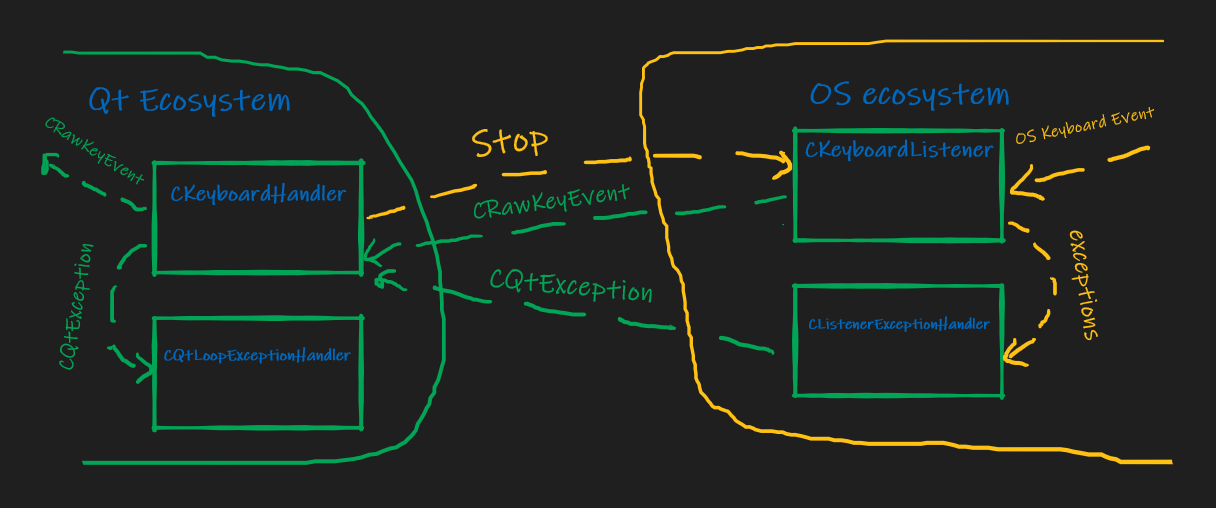
\includegraphics[scale = 0.5]{Figures/KeyboardInterception.png}

Green arrows represent queued Qt signals and yellow arrows represent OS dependent signals.
\end{center}

\subsubsection{AppStatus}

This object is a wrapper over the Qt application instance. It has observable values in terms of section~\ref{section::Observer}. It is currently used to react on switching between active and inactive states of the application. For example, I do not want to intercept keyboard, while the user interacts with the application GUI. Also, when user switch back to the application, we upload all intercepted sessions.


This object is a singleton according to section~\ref{section::Singleton}. It has one output sending the application current status. There are two options: active and inactive.

\subsubsection{SimdDetector}

This object determines the level of SIMD instructions available in run-time. It detects the level during construction time of the object and holds the value. Additionally, it disables subnormal numbers to speed up computations. According to the manual of the Vector Class Library by Agner Fog, many inline functions of the library do not support subnormal numbers. So, it is recommended to call \verb"no_subnormals".

This object is a singleton according to section~\ref{section::Singleton}. It provides one function \verb"level" to determine the level of accessible SIMD instructions.

\subsubsection{Parallel}

This object is capable of calling parallel algorithms. Its role is to simplify the access to different concurrent libraries. Currently, the following libraries are supported:
\begin{enumerate}
\item Inter TBB. Accessible on all platforms.
\item Microsoft Parallel Library. Windows only.
\item LibDispatch. (not implemented yet) Linux and Mac only.
\end{enumerate}
This object keeps the information on available libraries on the current machine, grants access to parallel algorithms of the current active library, and allows you to switch to a different available library in run-time.

This object is a singleton according to section~\ref{section::Singleton}.

\subsection{Kernel}


\subsubsection{Sessions and Seances}

When the application runs it uses a continuous time scale. Each new run of the application has its one time scale starting from zero. All key events on the same time line are grouped into a Seance. Each Seance can be separated into peaces called Sessions. The Session is considered as a peace of information to analyze. Each session is analyzed independently. When we load a file it contains key events on a different time scale. The notion of Seance allows us to separate current Seance intercepted while application is running and other Seances that are loaded from files.

The Seance is presented by \verb"CSeance" class. Currently this is an extension of \verb"std::deque" of \verb"CSession"-s (TO DO partially implemented). Session is presented by \verb"CSession" class. Currently this is an extension of \verb"std::vector" of \verb"CKeyEvent"-s. (TO DO partially implemented).


\subsubsection{CSeanceManager}

To understand \verb"CSeanceManater" and its responsibilities let us look on the following picture:
\begin{center}
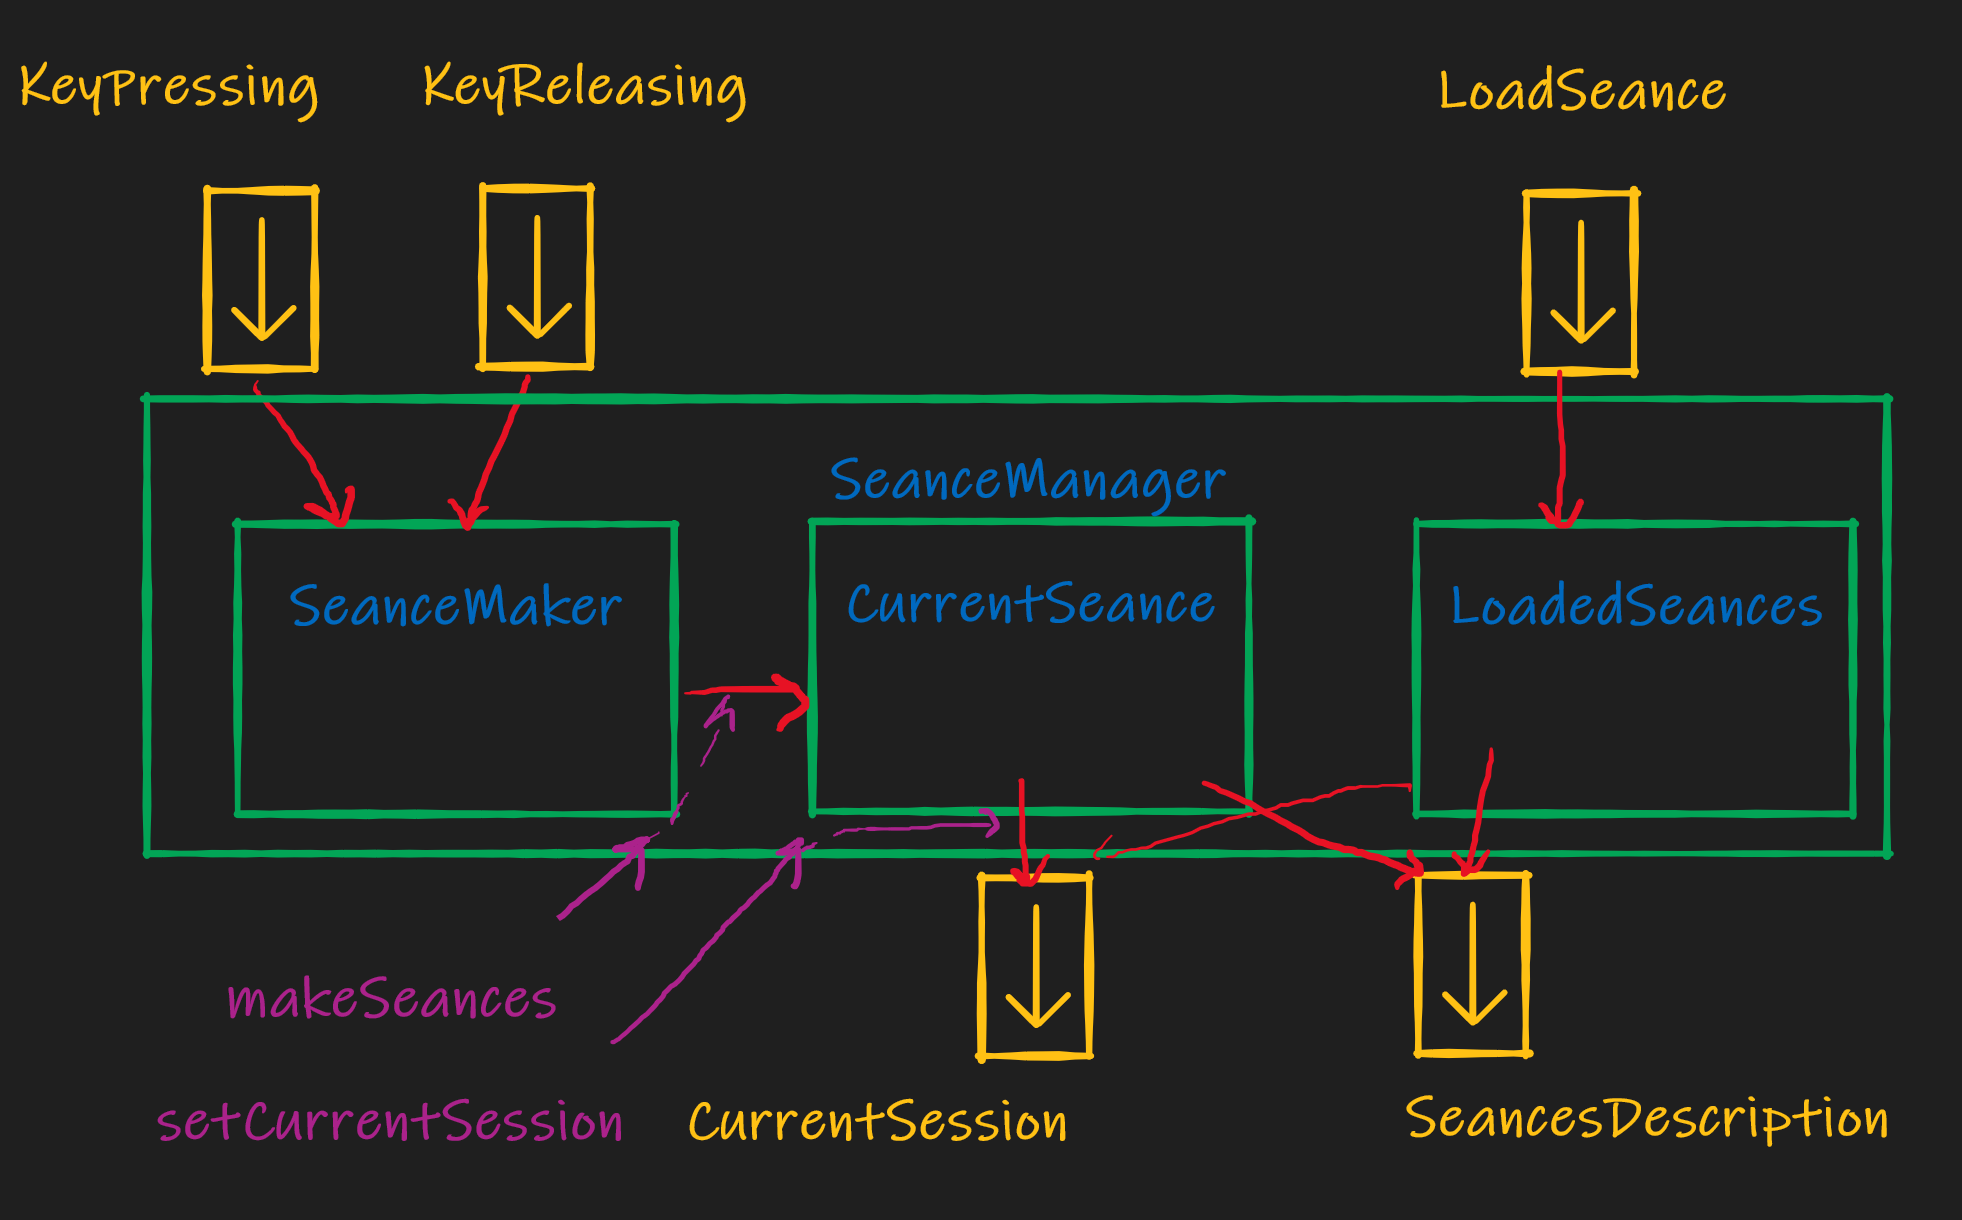
\includegraphics[scale = 0.4]{Figures/SeanceManager.png}

Green boxes represent objects. Yellow boxes are input/outputs according to the observer pattern. Violet arrows are methods to control the manager via MVC. Red arrows represent the data flow.
\end{center}

The manager has the following components:
\begin{enumerate}
\item \verb"SeanceMaker". This object receives key pressing and releasing events and store them in a raw form. It also divides the stored events into \verb"CRawSession"s. The \verb"CRawSession"s use \verb"std::list" container to have low cost modification actions.

\item \verb"CurrentSeance". Current seance stores all sessions intercepted by the application.

\item \verb"LoadedSeances". (TO DO not implemented yet) This object manages all loaded seances, e.g., loaded from files.
\end{enumerate}

The manager's responsibilities:
\begin{enumerate}
\item It receives Key Pressing and Key Releasing events from \verb"CKeyboardHandler" via observer pattern.

\item It receives new seances from a file loader (TO DO not implemented yet).

\item It returns current Seance to other parts of the application via observer pattern.

\item It returns current Seance and loaded Seances data (TO DO not implemented yet) via observer pattern. This is used by GUI to represent the set of seances visually.
\end{enumerate}

The manager has the following control options:
\begin{enumerate}
\item \verb"makeSessions". This method transforms \verb"CRawSession"s from \verb"SeanceMaker" to \verb"CSession"s, appends them to \verb"CurrentSeance", and clears the internal buffer, that is, \verb"CRawSeance".
\end{enumerate}

\paragraph{SeanceMaker}
This object eats \verb"CKeyPressing" and \verb"CKeyReleasing" events. It tries to pair pressing and releasing events to form \verb"CKeyEvent". Internally, \verb"SeanceMaker" contains \verb"RawSeance" that is \verb"std::list<CRawSession>" and \verb"CRawSession" is \verb"std::list<CKeyEvent>". There are several things you should be aware off:
\begin{enumerate}
\item If you press a key and hold it for some time, the key may generate artificial key pressing events in specific time intervals. The artificial key pressing events are marked by \verb"AutoRepeat" flag and do not have releasing time (releasing time is set to be zero). \verb"SeanceMaker" distinguishes the keys with autorepeat support and without. Currently autorepeat is not allowed for the shifters (left and right shift, alt, and ctrl and capslock).

\item The logic for division of \verb"CRawSeance" into \verb"CRawSession"s is the following. \verb"SeanceMaker" keep track the time of the last event and the keys that are being pressed currently. If the current \verb"CRawSession" is not empty, there are no pressed keys, and the time since the last event exceeds the time limit (if it is set) the new \verb"CRawSession" is opened. Currently, the time limit is set to be 10 seconds. (TO DO) In the future, there will be an option to set the time limit via application settings.
\end{enumerate}

\subsubsection{CSessionSelector}

This object selects one session in the seance. It sends the information about the seance and currently chosen session to \verb"CSeanceView" via observer pattern. \verb"CSeanceView" notifies \verb"CSeanceViewController" when the chosen session is changed in the widget by user. \verb"CSeanceViewController" sets new session. The objects \verb"CSessionSelector", \verb"CSeanceView", \verb"CSeanceViewController" are model, view, and controller, respectively.

\subsubsection{CTextModule}

\paragraph{General information}

This module receives the chosen session from \verb"SessionSelector". The module contains the following information:
\begin{enumerate}
\item \verb"CTextMode" is the information about currently chosen mode, i.e. raw session data, or printed text, or text with deleted symbols etc.
\item \verb"CTextDataTree" is a specific data structure required to identify mistakes in the text.
\end{enumerate}

\verb"CTextModule" notifies \verb"CTextModeView" about the state of the current text mode. \verb"CTextModeView" displays the state and notifies \verb"CTextModeController" whenever the state was changed. \verb"CTextModeController" sets new state in the \verb"CTextModule". The objects \verb"CTextModule", \verb"CTextModeView", and \verb"TextModeController" are model, view, and controller, respectively.

\paragraph{CVTree}

The text tree is based on \verb"CVTree" template. This structure represents a tree. Each node has five connections:
\begin{enumerate}
\item parent
\item first child
\item last child
\item previous sibling
\item next sibling
\end{enumerate}
and also contains some information in the node. The following picture shows an example of \verb"CVTree" .
\begin{center}
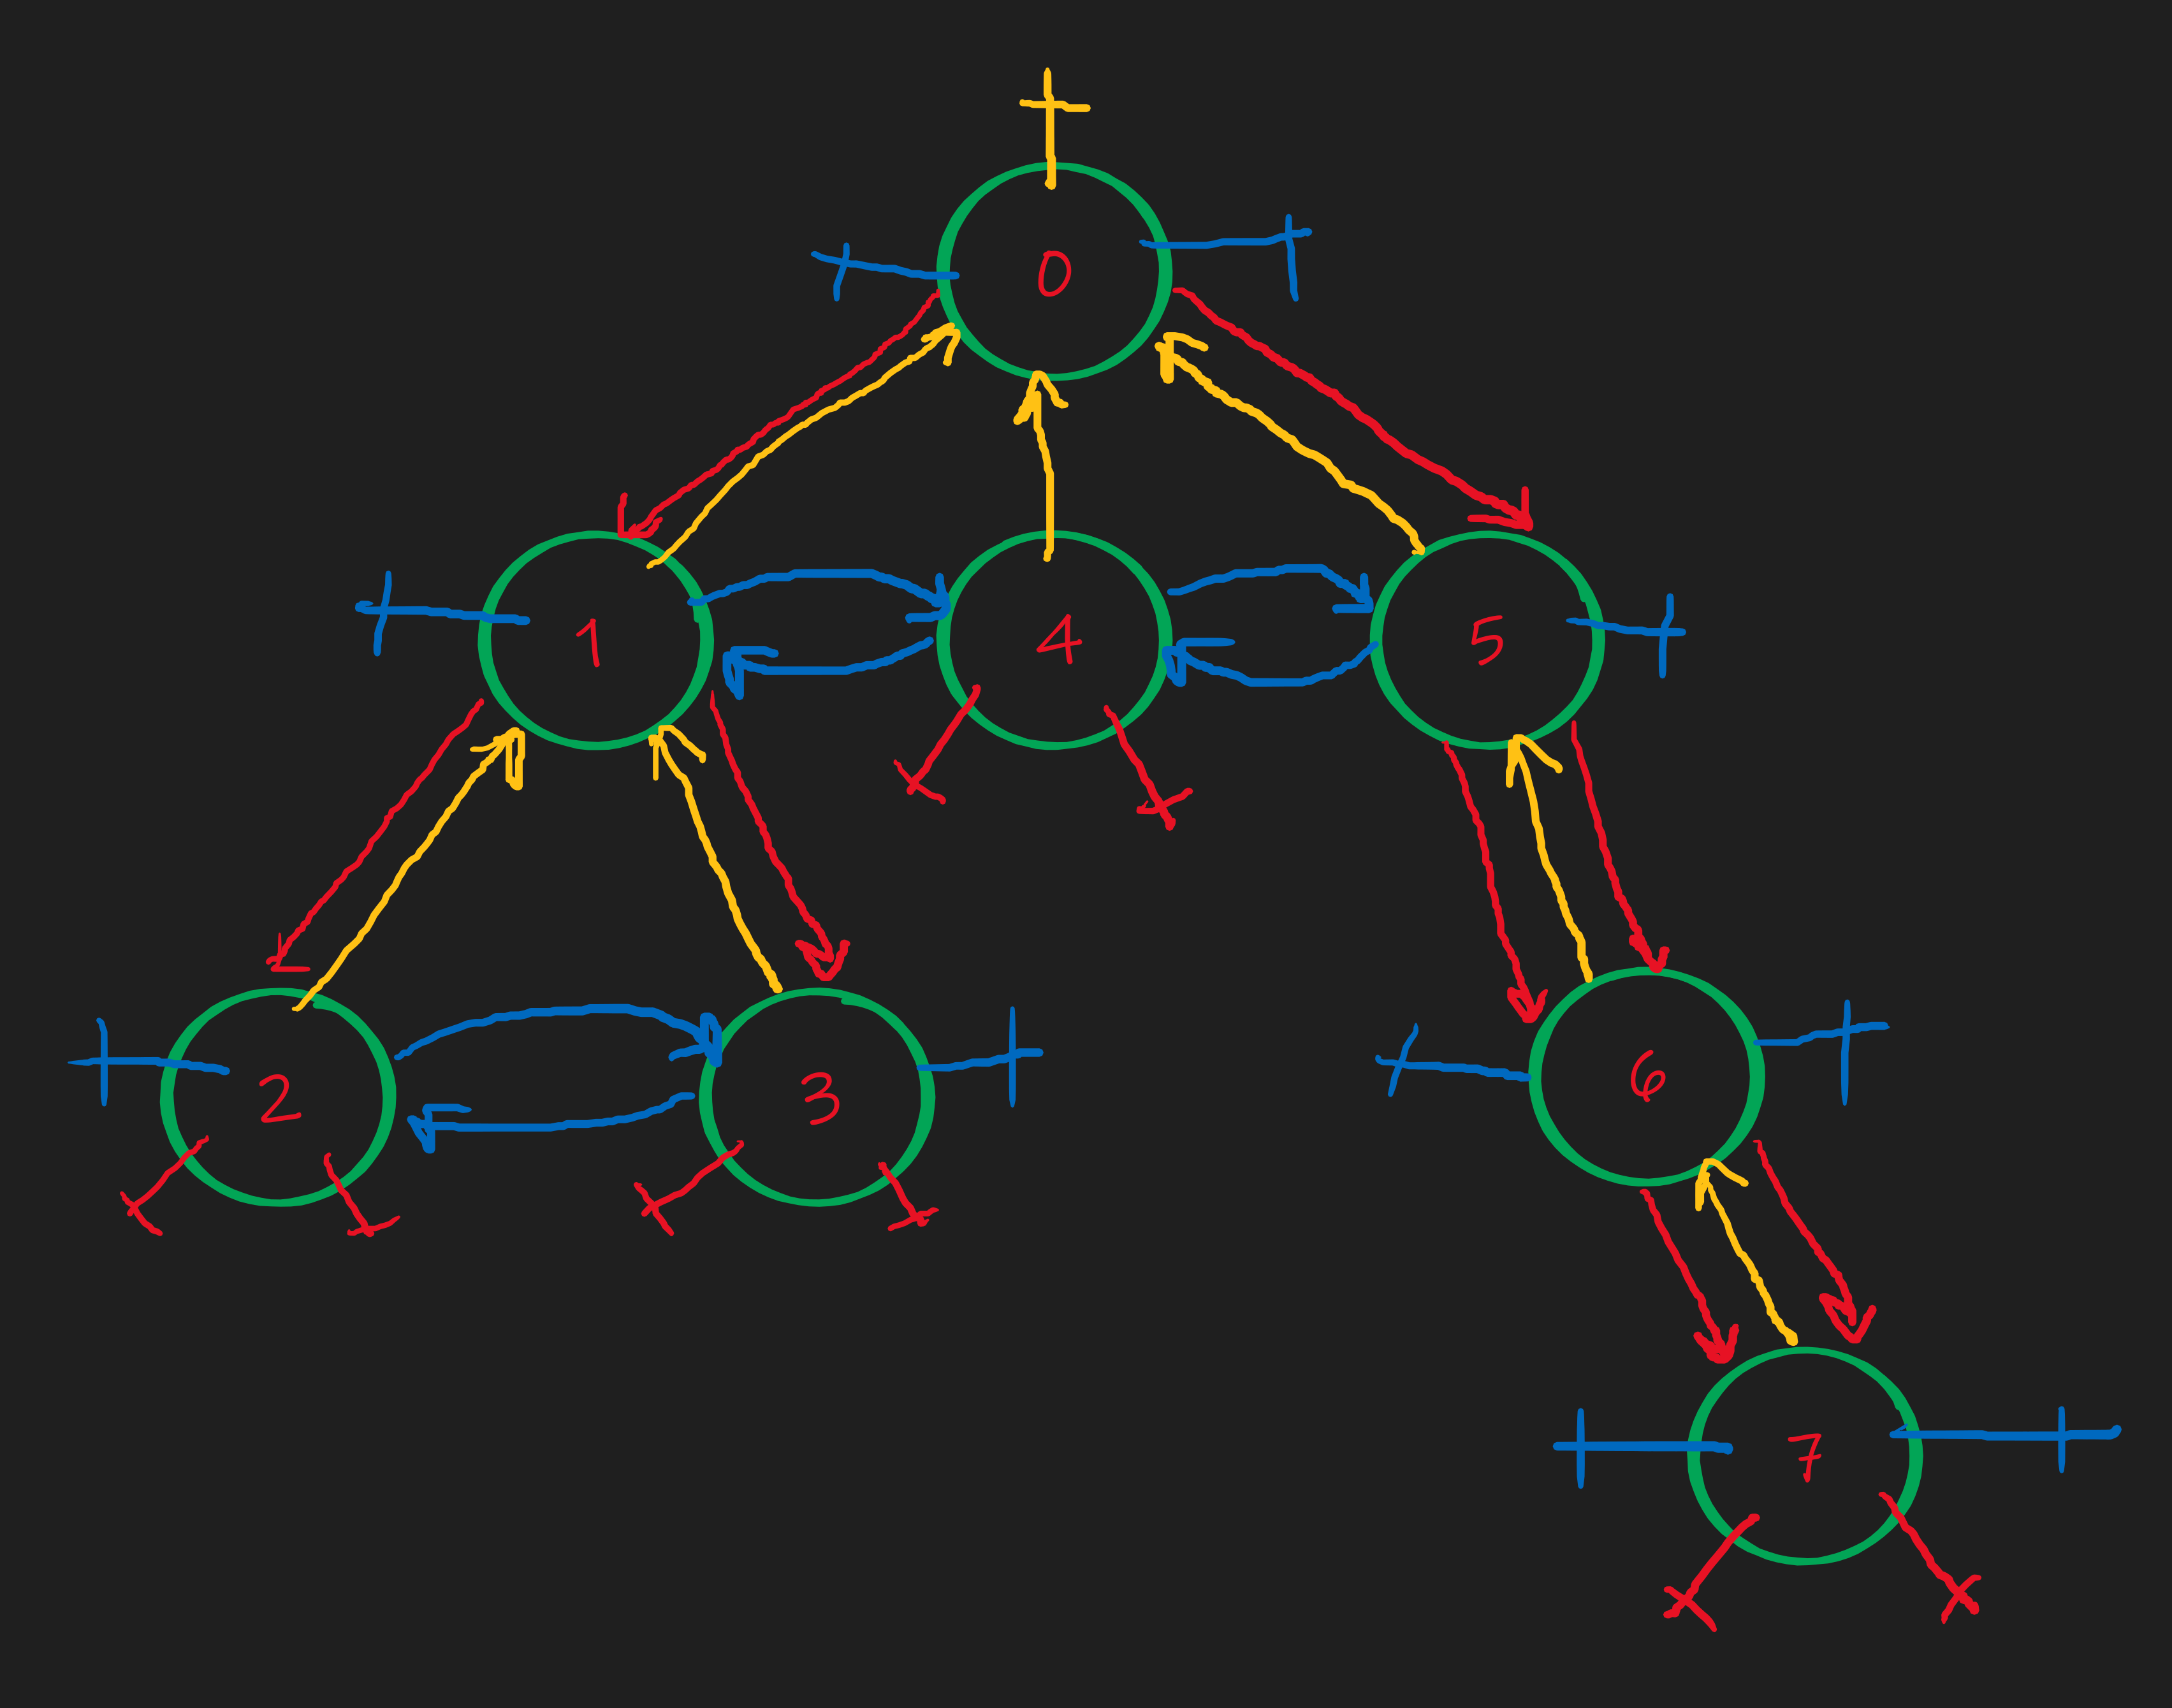
\includegraphics[scale = 0.2]{Figures/VTree.png}

Yellow arrows point to a parent, red arrows point to the first and last children, blue arrows point to the previous and next siblings.
\end{center}

In order to be efficient, the exact implementation uses \verb"std::vector". This results in some limitations:\footnote{I would like to use \textbf{std::pmr} and usual pointers in order to overcome these limitations.}
\begin{enumerate}
\item We cannot add and delete vertices in arbitrary places.
\item We can add to a vertex on the route from the root to the most right lief.
\item We can only add a last children to a vertex.
\end{enumerate}

The tree \verb"CVTree" supports three types of iterators:
\begin{enumerate}
\item PreOrder\footnote{The name was randomly chosen. I do not know how to name it properly.} iterators. The best way to discribe the order is the following: in order to print the tree you need print current vertex and then print all subtrees from left to right. The nodes on the picture are numbered according to this order.

\item LeftSon iterator. This iterators move on the right branch of the tree between the root and the most right lief.

\item Sibling iterator. This iterators are used to cycle through all the children of a vertex.
\end{enumerate}

\paragraph{CTextDataTree}

In order to track mistakes in the text we need a forest. Instead of dealing with a forest, we add a formal node as a new root and the forest become a tree. Here is an example:
\begin{center}
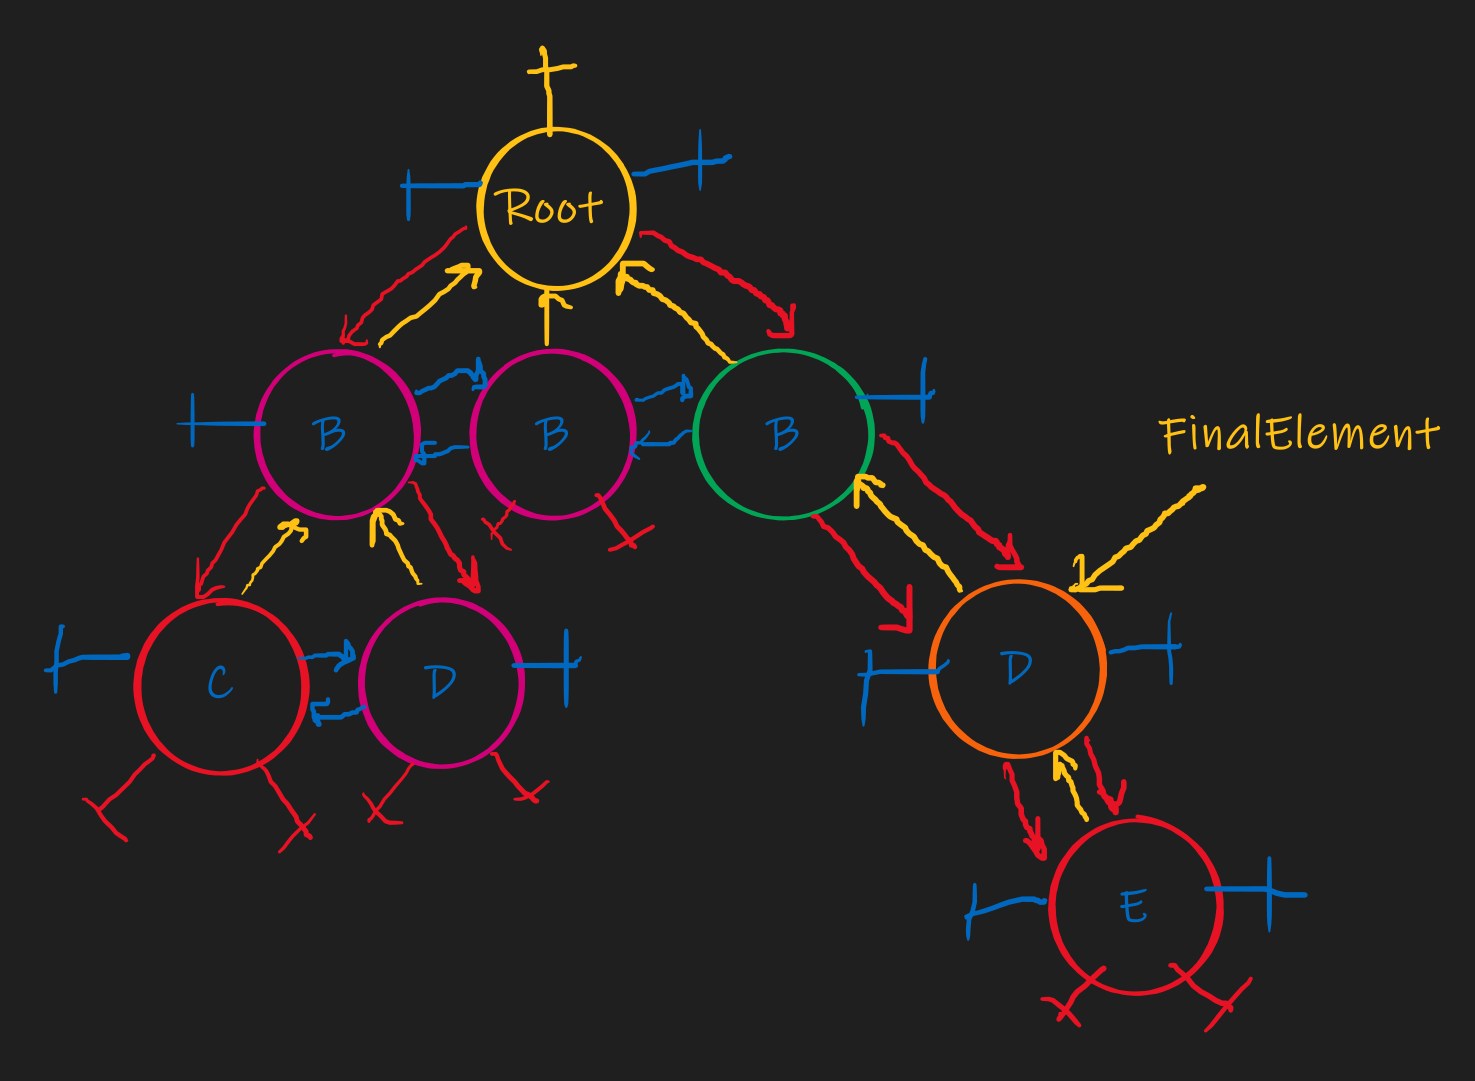
\includegraphics[scale = 0.4]{Figures/TreePrimitives3a.png}

An example of a \verb"CTextDataTree"
\end{center}

Suppose user types the following:
\begin{center}
\verb"BC[Backspace]D[backspace][backspace]B[Backspace]BDE[Backspace]"
\end{center}
The previous picture shows the structure of the corresponding \verb"CTextDataTree". However, it is more convenient to think of it as shown below (without all the pointers of the nodes):
\begin{center}
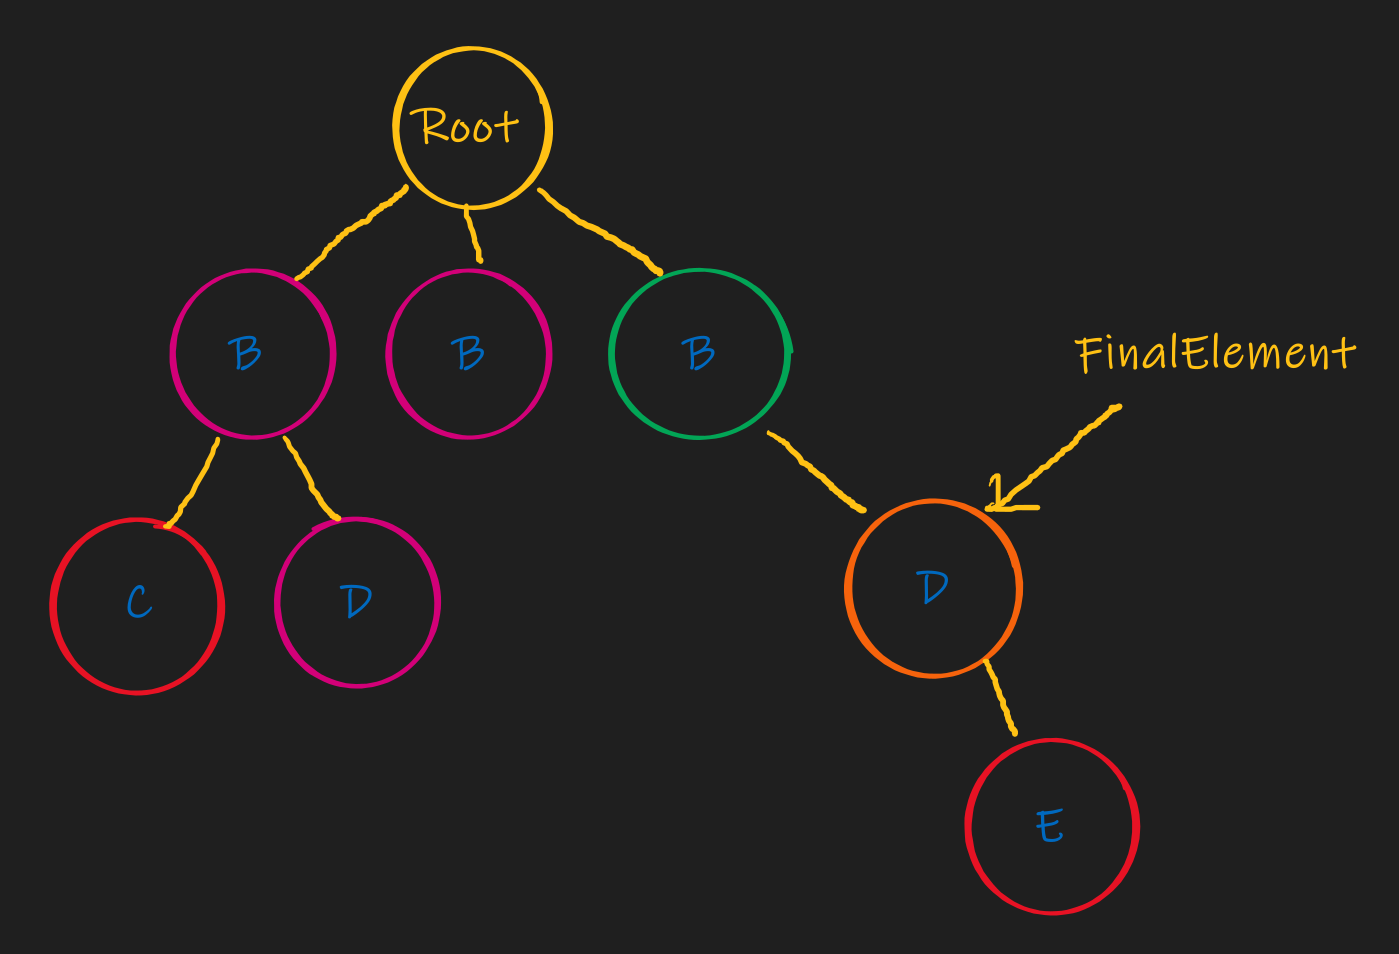
\includegraphics[scale = 0.4]{Figures/TreePrimitives4a.png}
\end{center}
As we can see the printed text correspond to the route from the root to the \verb"FinalElement" (a marked node in the tree). This route always goes through last child of each vertex. In the example above, printed text is
\begin{center}
\verb"BD"
\end{center}
Since we do not know the source text, we assume that the resulting text is the correct one, i.e. \verb"BD" is the correct text in this example. We compare everything with the printed text in order to find a mistake.

The vertices have the following states:
\begin{enumerate}
\item Yellow color. The root of the tree. This is an auxiliary node.
\item Green color. This color shows the regular text.
\item Orange color. This color shows where exactly a mistake happened.
\item Violet color. This color shows deleted symbols that need not be deleted, that is, if the user did not erase them, this would not lead to a mistake.
\item Red color. This color shows deleted symbols that were needed to be deleted in order to get a correct text.
\end{enumerate}
The algorithm for finding mistakes is the following:
\begin{enumerate}
\item We go from the root to the \verb"FinalElement" through last children.
\item For each node with two or more children we execute the following algorithm:
\begin{enumerate}
\item Take a route from the current node to a lief in its subtree.
\item Compare symbols in the route with the symbols in the printed text. 
\begin{itemize}
\item If the symbol is the same, this symbol is considered accidentally deleted and we move to the next one.
\item If symbol is different, we consider this place as a mistake. The symbol and all the remaining ones are considered as symbols required for deletion. The node in the printed text is marked as the place where the mistake happened.
\end{itemize}
\end{enumerate}
\end{enumerate}
Logically, we transform the tree into a different form as shown below:\footnote{The implementation of the exact procedure is a bit more sophisticated.}
\begin{center}
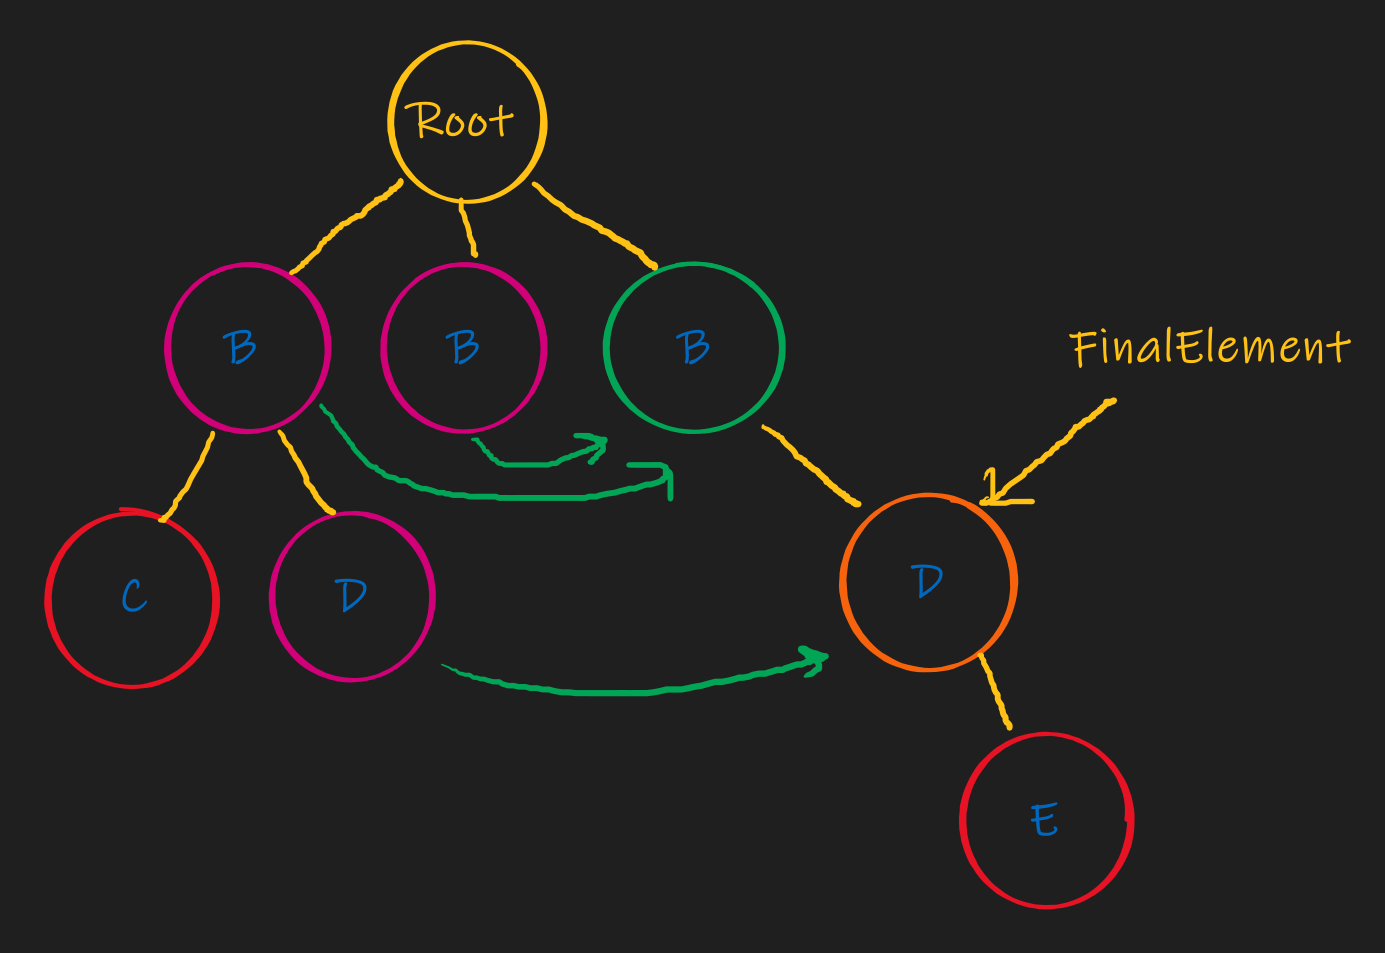
\includegraphics[scale = 0.4]{Figures/TreePrimitives5a.png}
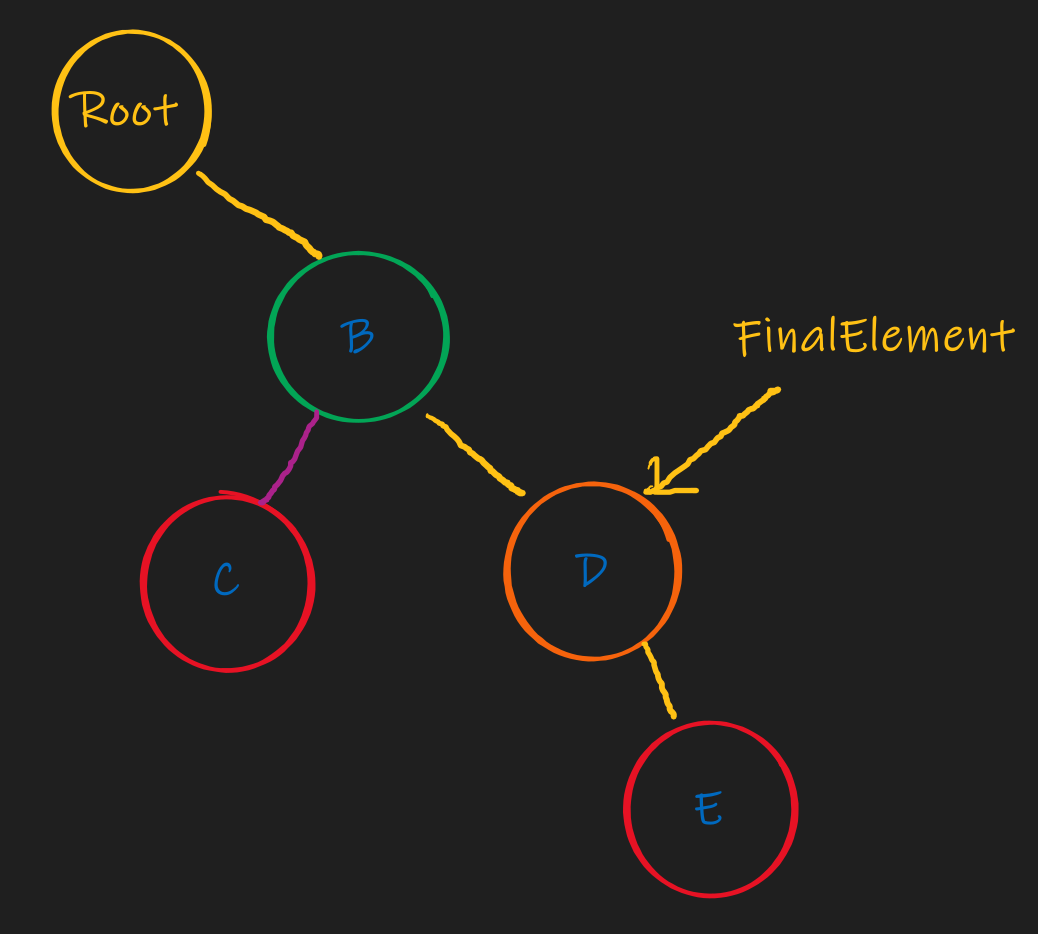
\includegraphics[scale = 0.4]{Figures/TreePrimitives6a.png}

Yellow node is the root. Green node shows the regular text. Orange nodes represent places where mistakes were done. Violet nodes show accidentally deleted symbols. Red nodes show deleted symbols that are required to be deleted.
\end{center}
After this transformation, every node with more than one child is the symbol preceding a mistake. Al elements after \verb"FinalElement" are considered as mistakes (red nodes). This approach allows to find all the mistakes as well as how many times the mistake was done in a particular place. As a result, we can analyze the distribution of the mistakes.

\paragraph{Text Mode}

Currently there are three different text modes:
\begin{enumerate}
\item Raw output
\item Full text
\item Printed text
\end{enumerate}
The Raw output shows each key in the session, Full text shows printed text including all deleted symbols, Printed text shows only final text without deleted symbols. The following examples illustrate the output for the tree from the previous section:
\begin{center}
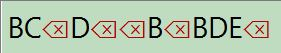
\includegraphics[scale = 0.6]{Figures/raw_session.jpg}
\quad
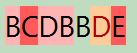
\includegraphics[scale = 0.6]{Figures/full_text.jpg}
\quad
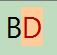
\includegraphics[scale = 0.6]{Figures/printed_text.jpg}

1) The first figure shows the Raw output. Here you can see the labels of the keys. 2) The second figure shows all the symbols printed and deleted ones. Black symbols on the green background represent the usual text. Orange background corresponds to a symbol where a mistake appeared. Pink and red colors represent deleted symbols. The red ones are the symbols that were required to delete. The pink ones are the symbols that did not lead to a mistake. The user did not need to delete them. 3) The latter mode is Printed text. It shows the final text.
\end{center}

\subsubsection{Analytical Module}

The aim of the module is to extract information from the \verb"CTextData" came from \verb"CTextModule". Currently it extracts:
\begin{enumerate}
\item Density of the speed distribution.
\end{enumerate}

\paragraph{CFunctionData}

This object hold required information to compute density of random variable. It contains
\begin{enumerate}
\item Samples. Data samples of the random variable, i.e. if the random variable is the speed of typing, then Samples contain the values of the speed of each key.

\item Plot Data. This object contains the information required to draw the required plots.
\end{enumerate}

\paragraph{CPlotData}

Computation of the plots is the most time consuming place of the application. \verb"CPlotData" stores inside the values of $x$-coordinates for the grid to draw plots and $y$-values on the grid for each plot.


Currently there are three different methods to approximate the densities:
\begin{enumerate}
\item Approximation using normal distribution. 
\item Approximation using Maxwell-Boltzmann distribution.
\item Approximation using Rayleigh distribution.
\end{enumerate}

\begin{center}
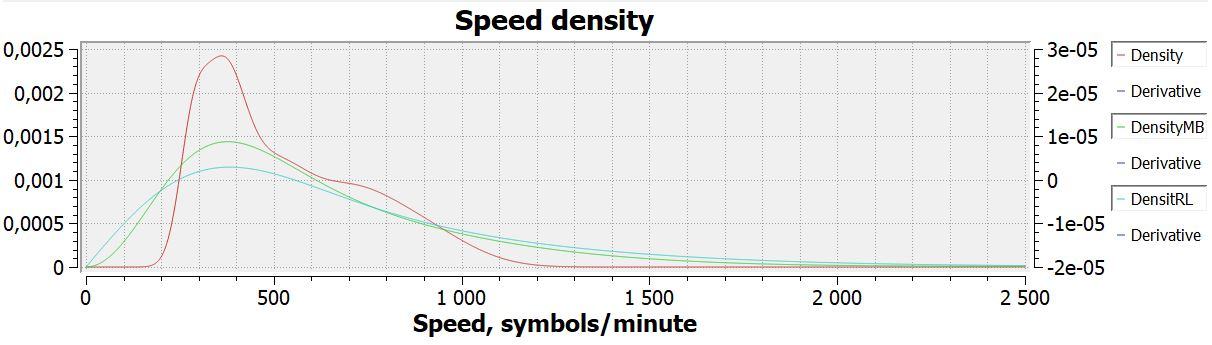
\includegraphics[scale = 0.6]{Figures/Density.jpg}

The red color plot is the approximation using normal distribution, the green color plot is the approximation using Maxwell-Boltzmann distribution, and the blue color plot is the approximation using Rayleigh distribution.
\end{center}
\begin{center}
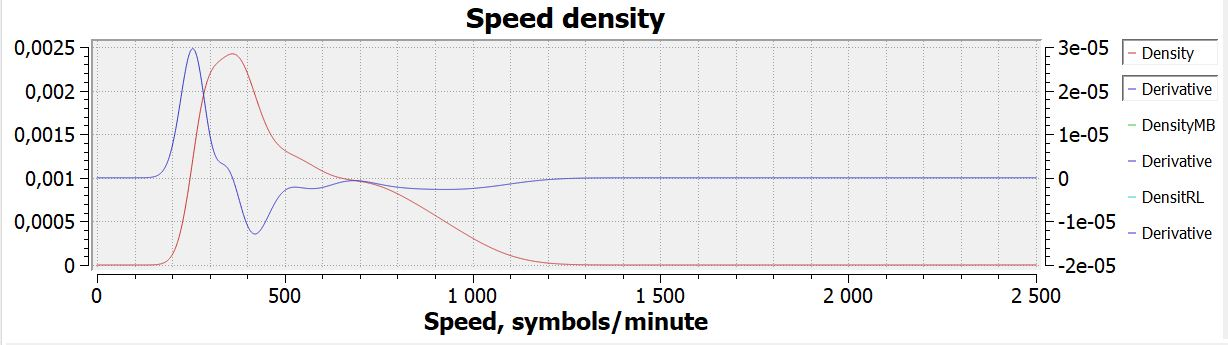
\includegraphics[scale = 0.6]{Figures/DensityAndDerivative.jpg}

Here you can see the plots of the approximation using normal distribution and its derivative. The axis for the approximation is on the left and the axis for the derivative is on the right.
\end{center}

\paragraph{CMath}

The computation is delegated to the \verb"CMath" object. \verb"CMath" is a singleton. It tries to initialize CUDA device if possible and uses it for the computation. If CUDA device is not accessible it uses CPU. \verb"CMath" uses multiple threads and SIMD optimizations.

The objects computing density or its derivative on CPU use Samples and an argument. Internally each such an object uses SIMD to speed up the computation. Currently SSE2 and AVX levels are used. The level SSE2 is default for x64 systems and allows to operate with $2$ doubles at the same time. The level AVX allows to operate with $4$ doubles at the same time. The level of instructions is determined in run-time by special object \verb"SimdDetector". In order to deal with SIMD instructions, Vector Class Library of Agner Fog is used.

Each object computing the density on CPU is based on \verb"FunctionModuleBase" template. The template simplifies the dispatching of functions for different SIMD levels.

In order to fill a plot grid on CPU we use \verb"parallel_for" algorithm. The following parallel libraries are used:
\begin{enumerate}
\item Inter TBB. Accessible on all platforms.
\item Microsoft Parallel Library. Windows only.
\item LibDispatch. (not implemented yet) Linux and Mac only.
\end{enumerate}
In order to simplify the usage of the libraries, we use a wrapper \verb"CParallelModule". This module keeps the information on available libraries on the current machine, grants access to \verb"parallel_for" algorithm of the current active library, and allows you to switch to a different available library in run-time.

\subsubsection{UserData Module}

The purpose of the module is to store user specific information. Currently it contains user's Finger Layout. It maps fingers to physical keys. Currently, the layout is not modifiable.

\subsubsection{KeyScheme Module}

The purpose of the module to produce a key scheme for the current text regime. The key scheme is a graphical representation of keys on a time-line. It shows which key was pressed by which finger and the text the key generated (or a key label).
\begin{center}
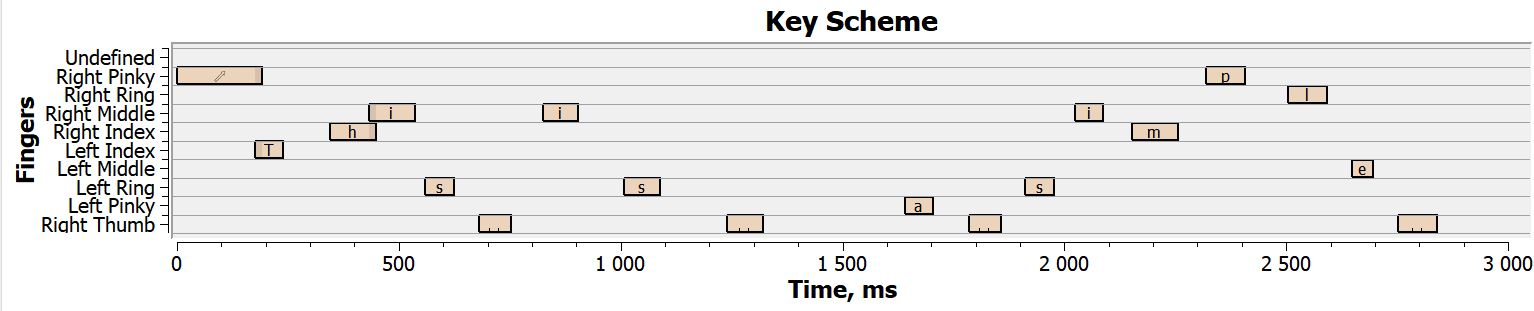
\includegraphics[scale = 0.6]{Figures/KeyScheme.jpg}

An example of a Key Scheme.
\end{center}
If the keys  are overlapped the corresponding zone is colored in a darker shade of the key color. The the more keys are pressed simultaneously the darker the shade.
\subsection{Qt Resources}

\subsection{ApplicationImpl}

There are currently the following control elements:
\begin{enumerate}
\item \verb"KeyboardShutter". This object listens to the application status. If application becomes active it shuts down the keyboard interception. When application becomes inactive it turns the keyboard interception on.

\item \verb"SessionFlusher". This object listens to the application status. If application becomes active it flushes intercepted sessions currently stored in the buffer of \verb"SeanceManager".
\end{enumerate}



\section{Debugging}\label{section::Debugging}

In order to turn on debugging options, you need to define a macro in \verb"TypeingAnalysis.pro" file. Currently the following macros are available:
\begin{enumerate}
\item \verb"KEYBOARD_HANDLER_DEBUG"
\end{enumerate}

When you comment or uncomment a macro in the pro file you will probably need to go through: clear, run qmake, and rebuild sequence.

\paragraph{KEYBOARD\_HANDLER\_DEBUG}

This macro activates an additional window showing the data received by the Keyboard Handler of the application. Currently it is connected to key pressing and releasing events of the handler and prints the messages information. The connection is done via Observer pattern~\ref{section::Observer}. The debug window closes automatically when the main window is closing.

\section{Code}

\section{Implementation}

\section{Library}
\subsection{Singleton}\label{section::Singleton}
CAnyGlobalAccess template consists of three parts:
\begin{enumerate}
\item \textbf{CAnyGlobalAccessible}. It provides a static storage for a global object. You do not access it directly.
\item \textbf{CAnyGlobalAccess}. This object is used to access the global object. The global object must be initialized before access object is created.
\item \textbf{CAnyGlobalInitializer}. This object is used to initialize the global object. You need to create one instance of this object in order to initialize the global object.
\end{enumerate}
\begin{center}
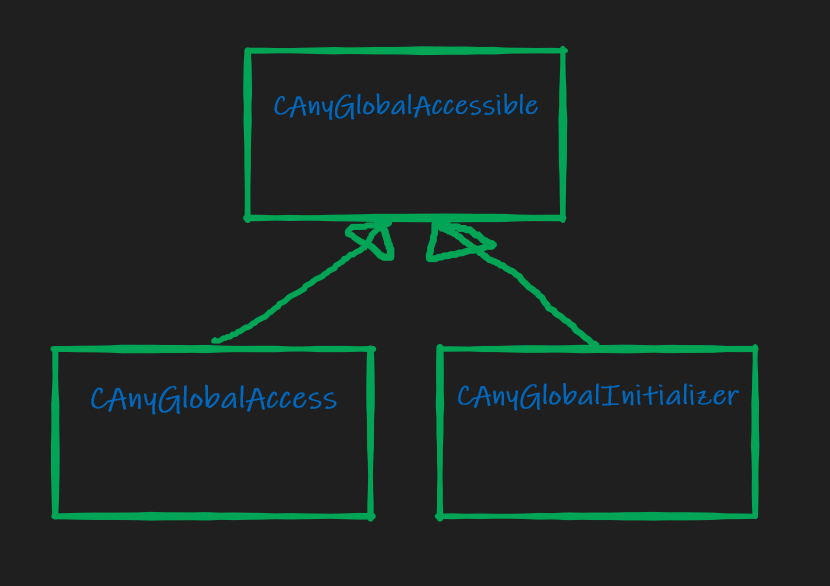
\includegraphics[scale = 0.3]{Figures/CAnyGlobalAccess.png}
\end{center}

\paragraph{Description}
The pattern is used to make a global object with non-trivial constructor without explicitly defining the object globally. \textbf{WARNING} this thing is NOT thread safe! In order to use the pattern we must provide:
\begin{enumerate}
\item \verb"TAccessible" -- the class for the global object

\item \verb"TID" -- identification class. If we want to have several global objects  of a class Type, we must distinguish them by a dummy class \verb"TID". For example, \verb"CAnyGlobalAccessible<Type, A>" and \verb"CAnyGlobalAccessible<Type, B>" store  different instances of objects of type Type in static storage. Since static objects defined by the class they belong to, classes \verb"A" and \verb"B" are required to distinguish the instances.

Example of a dummy class declaration:
\begin{verbatim}
class CGlobalAccessibleID;
\end{verbatim}

\item A class for initialization of the global object. It must be
 inherited from \verb"CAnyGlobalInitializer". The class must inherit all the constructors of the base class.
\begin{verbatim}
class CMyInitializer : CAnyGlobalInitializer<TAccessible, TID> {
   using CBase = CAnyGlobalInitializer<TAccessible, TID>;
 public:
   using CBase::CBase;
 };
\end{verbatim}

\item A class for getting access to the global object must be publicly inherited from \verb"CAnyGlobalAccess". It has only a default constructor. It asserts if  the global object has not yet been initialized.
\begin{verbatim}
class CMyAccessor : public CAnyGlobalAccess<TAccessible, TID> {};
 \end{verbatim}
\end{enumerate}

\paragraph{Example}
Suppose we want a global \verb"int" variable for logging:
\begin{verbatim}
class CLoggerCounterID;
class CLoggerCounterInitializer :
  CAnyGlobalInitializer<int, CLoggerCounterID> {
  using CBase = CAnyGlobalInitializer<int, CLoggerCounterID>;
public:
  using CBase::CBase;
};
class CLoggerCounterAccess : public CAnyGlobalAccess<int, CLoggerCounterID> {};
\end{verbatim}
Then in code we write something like that:
\begin{verbatim}
...
CLoggerCounterInitializer Init(0);
...
CLoggerCounterAccess LogCounter;
++(*LogCounter);
std::cout << *LogCounter << std::endl;
...
\end{verbatim}

\subsection{AnyObject}
\subsubsection{AnyMovable}\label{section::AnyMovable}

\paragraph{Description}
\verb"CAnyMovable" allows you to store any movable only class without any restrictions on the class. It also allows you to provide  an interface to a class and implementations for different classes of the method.

The \verb"operator->()" goes without any checks and may fail if the object is empty, that is, does not store anything. It is your responsibility to call \verb"isDefined()" method before accessing the interface.

The class \verb"CAnyMovable" does not use Small Object Optimization. In particular, move operations are always cheap. \verb"CAnyMovable" has value semantics and extends the ideas of Sean Parent's talk on cppcon about Run-time Polymorphism.

\paragraph{How to use}
In order to use the template you need:
\begin{enumerate}
\item Create an interface class:
\begin{verbatim}
template<class TBase>
class IAny : public TBase {
public:
  virtual void print() const = 0;
};
\end{verbatim}
The class describes the interface of an abstract object you want to support. Do not use names with prefix underscore here, e.g.,
\begin{itemize}
\item[\textbf{BAD}:] \verb"virtual void _print() const = 0;"
\item[\textbf{GOOD}:] \verb"virtual void print() const = 0;"
\end{itemize}
This interface will be accessible when using \verb"operator->()" on \verb"CAnyObject". The example is below.

\item Create an implementation class:
\begin{verbatim}
template<class TBase, class TObject>
class CAnyImpl : public TBase {
  using CBase = TBase;
public:
  using CBase::CBase;
  void print() const override {
    std::cout << "data = " << CBase::Object() << std::endl;
  }
};
\end{verbatim}
Here you implement all the functions from the interface. The parameter \verb"TObject" is used to reimplement the behaviour for different types of objects if needed. In the example above, it may happen that \verb"TObject" does not support stream \verb"operator<<" and you want to define  a specialization of the implementation class. Access to the stored object is provided by the method \verb"CBase::Object()".

\item Create your Any class:
\begin{verbatim}
class CAny : public CAnyMovable<IAny, CAnyImpl> {
  using CBase = CAnyMovable<IAny, CAnyImpl>;
public:
  using CBase::CBase;
  friend bool operator==(const CAny&, const CAny&) {
    ...
  }
};
\end{verbatim}
You can add any additional functionality to your \verb"CAny" class.
\end{enumerate}
Now you can use it like this:
\begin{verbatim}
CAny x = 'c';
x->print();
x = std::move("123");
x->print();
x = 1.45;
x->print();
\end{verbatim}
If you want to store an object of Type \verb"R" and construct it on the fly from the data: \verb"x, y, z". Then use emplace function or emplace constructor like this:
\begin{verbatim}
CAny s;
s.emplace<R>(x, y, z);
CAny y(std::in_place_type_t<R>(), x, y, z);
\end{verbatim}
Then the object of type \verb"R" will be created without creation of intermediate objects.

\paragraph{Implementation}
Internally \verb"CAnyMovable" stores an \verb"std::unique_ptr" to interface \verb"IObjectStored". Let us look at the diagram below:
\begin{center}
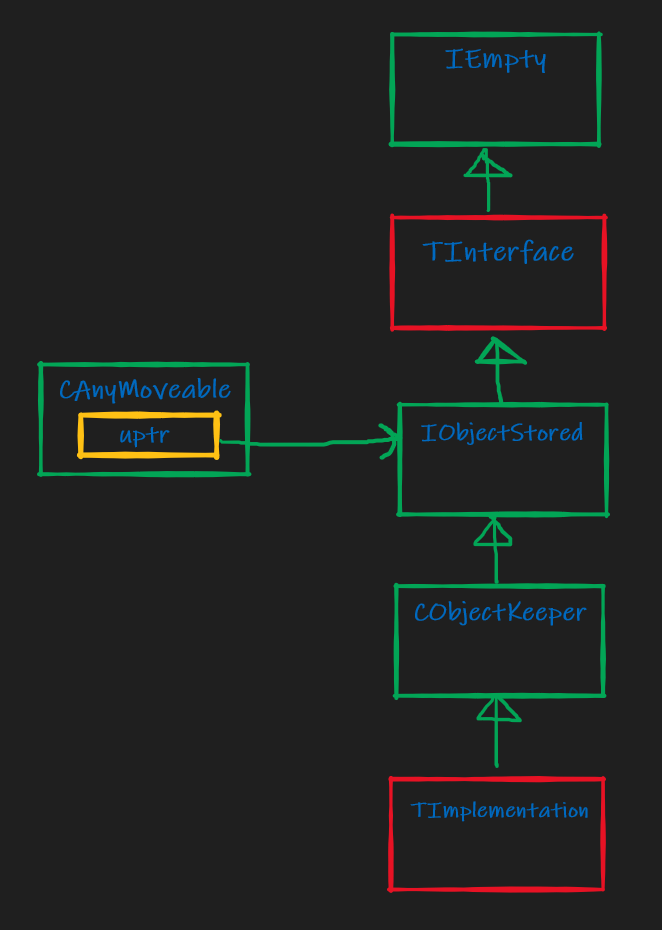
\includegraphics[scale = 0.5]{Figures/CAnyMovable.png}
\end{center}
The red rectangles are templates provided by the user. \verb"IEmpty" is an empty interface with virtual distructor. Its only purpose is to avoid user having to provide a virtual distructor in the \verb"TInterface" template. Then \verb"IObjectStored" adds some virtual methods to provide required functionality. \verb"CObjectKeeper" is a template storing an instance of an object you want to move into \verb"CAnyMovable". \verb"TImplementation" is a user defined template implementing all virtual methods from \verb"TInterface".

\subsection{Observer}\label{section::Observer}

% TO DO
% Need to update this

\paragraph{Description} The library provides several primitives to use Observer pattern. The most basic primitives are:
\begin{enumerate}
\item \verb"CObservable<TData>"
\item \verb"CObserver<TData>"
\item \verb"CSource<TData>"
\end{enumerate}

All primitives are synchronous. Observable notify events return after all its observers perform their actions.

All these objects are addressable. This means you must follow the rules for addressable objects. Usually this means you put this objects into unique pointer or inside other addressable object. Never store addressable objects in a vector or on the stack.

\paragraph{Observable}
\verb"CObservable<TData>" is an observable value of type \verb"TData". The Observable need not to contain the data. Instead, it has a method to get access to the data. You may provide such a method in the constructor. \verb"CObservable<TData>" provides the following methods:
\begin{enumerate}
\item \verb"subscribe(CObserver<TData>*)". This method subscribe an observer to the observable. The observable may have many subscribed observers. When you subscribe an observer that is already subscribed, the observer is unsubscribed first (even if this is the same observable). On subscription, every observable is put into the end of the list of subscribers. This is indeed an \verb"std::list<CObserver<TData>*>".

\item \verb"notify()". This method notify all subscribed observers about the data change. The subscribers are notified in the order they are presented in the list of the subscribers.
\end{enumerate}

There are three types of notifications from \verb"CObservable<TData>"
\begin{enumerate}
\item Notification on subscribe.
\item Notification on calling \verb"notify()".
\item Notification on unsubscribe.
\end{enumerate}
An observer may and can react differently in all three cases.

\paragraph{Source}

The observer pattern allows you to pass undefined data via std::optional. If TData is one of the following
\begin{enumerate}
\item arithmetic type
\item pointer type
\item enum type
\end{enumerate}
then it is passed by value and all other types are passed by const reference. In this case \verb"isPassedByValue" variable is set to true. In order to deal with these variety of cases in a convenient way, the library provides \verb"CSource<TData>" class. This class is used internally inside a connection between an observer and an observable. An observer get data from observable through an object of type \verb"CSource<TData>". The source object does not store the data, instead it has an action that returns the data. You may provide the action in the constructor. If you do not provide the action, the source will return undefined data. All methods are safe. You do not need to worry about run-time errors. Undefined data is handled with \verb"std::optional" on a regular basis.

\verb"CSource<TData>" has the following type aliases
\begin{enumerate}
\item \verb"CReturnValueType". If \verb"TData" is passed by value, then \verb"CReturnValueType" is equal \verb"TData" otherwise it coincides with \verb"std::reference_wrapper<const TData>".

\item \verb"CGetType". This is the type return by \verb"CSource<TData>" object. It is defined as \verb"std::optional<CReturnValueType>". This allows to handle the case of no data passing from the observable if the data is not defined at the moment.

\item \verb"CGetSignature". This is the signature of the action returning a value from the source.

\item \verb"CGetAction". This is the type of the action returning a value from the source.
\end{enumerate}

\verb"CSource<TData>" has the following methods:
\begin{enumerate}
\item \verb"hasGetter". This check if the source has a getter action returning a value.
\item \verb"operator()" or \verb"get()". These methods are synonymous and return the value of \verb"CGetType" an observer. This actions are safe to call even if the getter is not defined. In the latter case the result of static \verb"getNothing" action is returned.
\item \verb"set(CGetAction)". This method allows to change the source getter action.
\item \verb"Getter()". This method return the getter action by value. It is safe to call this method even if the action is not defined. In this case the static \verb"getNothing" action is returned.
\item \verb"hasValue()". This method checks if the source returns a well-defined value. It returns true only if the action is defined and the action returns a well-defiled value, that is, the optional indeed has a value.

\item static \verb"getNothing()". This is a static default getter action returning undefined optional as a result.
\end{enumerate}

\paragraph{Observer}

\verb"CObserver<TData>" is an observer of a value of type \verb"TData". The observer contains three actions to react to an observable notifications. You must provide them in the constructor of the observer. Each observer can be subscribed to at most one observable.

\verb"CObserver<TData>" provides the following methods (all methods are safe to call in any state):
\begin{enumerate}
\item \verb"isSubscribed()". Checks if the observer is subscribed to an observable.
\item \verb"hasValue()". Checks if the observer has a source returning a well-defined value, that is, the observer is subscribed to an observable and the observable provides a well-defined value (the optional result has a value).
\item \verb"data()". Returns a value from the connection with observable. If not connected, the result is the undefined optional.
\item \verb"Getter()". Returns the getter action of the connection with an observable. Returns \verb"getNothing" default action if not connected.
\item \verb"unsubscribe()". Unsubscribe from the current observable if any.
\item \verb"setSubscribe(CMethod)". This methods changes the action on subscription.
\item \verb"setNotify(CMethod)". This method changes the action on notification.
\item \verb"setUnsubscribe(CMethod)". This method chages the action on unsubscription.
\end{enumerate}

\paragraph{Higher level primitives} The library provides higher level observable and observers. Currently the following are implemented:
\begin{enumerate}
\item \verb"CObservableData<TData>"
\item \verb"CNotifier"
\item \verb"CObserverStrict<TData>"
\item \verb"CObserverHot<TData>"
\item \verb"CObserverCold<TData>"
\item \verb"CObserverHotStrict<TData>"
\item \verb"CHotInput<TData>"
\item \verb"CObserverColdStrict<TData>" or  \verb"CColdInput<TData>"
\item \verb"CHotActiveInput<TData>"
\item \verb"CColdActiveInput<TData>"
\end{enumerate}

\begin{itemize}
\item \verb"CObservableData<TData>" contains data of type \verb"TData" (the type must be an appropriate type that can be stored in \verb"std::optional"). It has a method to change the data and notifies the observers immediately after the change.

\item \verb"CNotifier" this is \verb"CObservable<void>". It is used when you need to send a dataless signal to an observer.

\item \verb"CObserverStrict<TData>" this is an observer reacting to notifications only in case the data is well-defined, that is, when the optional value sent by an observable has a value.

\item \verb"CObserverHot<TData>". This is an observer reacting on subscribe and notify events and doing nothing on unsubscribe event.

\item \verb"CObserverCold<TData>". This is an observer reacting on notify event only and doing nothing otherwise.

\item \verb"CObserverHotStrict<TData>". This observer behaves like the hot observer and reacts only on well-defined data.
\item \verb"CHotInput<TData>". This \verb"CObserverHotStrict<TData>" with the same actions for subscription and notification events.

\item \verb"CObserverColdStrict<TData>" or \verb"CColdInput<TData>". This is cold observer that reacts on well-defined data only.

\item \verb"CHotActiveInput<TData>". This observer can be in two states: active or inactive. It has one action. When the observer is subscribed or notified, if the data from the observable is well-defined, it becomes active and reacts using the action it has. When the observer is unsubscribed it becomes inactive. It also has a method \verb"deactivate()" to make it inactive. You can check its status using \verb"isActive()" method.

The use case. This input is useful when you want to treat the input as an instance of something. So, when you get a well-defined data the input becomes active, that means it "holds the data from the observable". When you read the data from the input, you set it to inactive state to simulate "the value is consumed" process.

It is also useful when you need to subscribe different inputs to the same observable and react only once when both inputs get their values.

\item \verb"CColdActiveInput<TData>". This observer can be in two states: active or inactive. It has one action. When the observer is subscribed it does nothing. When observer is notified, if the data from the observable is well-defined, it becomes active and reacts using the action it has. When the observer is unsubscribed it becomes inactive. It also has a method \verb"deactivate()" to make it inactive. You can check its status using \verb"isActive()" method.
\end{itemize}

The use case is similar to the one for the hot version. It allows you to ignore the subscription event in the similar scenarios.

\paragraph{How to use}

Here is an example of usage:
\begin{verbatim}
void print_sub(int x) {
  std::cout << "sub value = " << x << std::endl;
}
void print_not(int x) {
  std::cout << "not value = " << x << std::endl;
}
void print_unsub(int x) {
  std::cout << "unsub value = " << x << std::endl;
}
CObservableData<int> value;
CObserverStrict<int> printer(print_sub, print_not, print_unsub);
value.subscribe(&printer);
value.set(1);
value.set(2);
\end{verbatim}

In this example all the objects are created on stack. However, you must not do that. If you need to create an observer or observable, either use \verb"std::unique_ptr" to hold them or create them inside another addressable object.

\paragraph{Remarks}

(TO DO) Need to implement value semantics wrappers for the primitives to avoid explicit using of \verb"std::unique_ptr" all the time. The wrapper will be a movable object.

\end{document}


